\section{Fluxograma do Tableau}
\subsection{Problema de Maximização}

\begin{frame}
\frametitle{Fluxograma Tableau Simplex - \color{pink!100} MAXIMIZAÇÃO}
	\centering
	\begin{tikzpicture} [
							auto, node distance = 2cm,
							decisao/.style = { diamond, draw, shape aspect=2, thick, fill=red!20,
							                   text width=6em, text badly centered,
							                   inner sep=1pt},
							bloco/.style   = { rectangle, draw, thick, fill=blue!20, 
												text width=5em, text centered,
							                   minimum height=1em },
							bloco2/.style   = { rectangle, draw, thick, fill=blue!20, 
												text width=5em, text centered,
							                   minimum height=1em, node distance = 4.2cm },
							extremo/.style  = { ellipse, draw, fill=green!20,
							                   text width=5em, text centered,
							                   minimum height=2em },	
							line/.style   = { draw, -latex' },
							goto/.style = {circle, draw, fill=yellow!60, text width=1em,
										   text centered, node distance = 1.8cm},
						    bullet/.style = {rectangle, draw, thick, fill=red!80, 
						    				text width=9em, text centered,
						    				minimum height=1em},
						]

	
		\node [extremo] (inic) {\tiny INÍCIO}; \pause
		
		\node [bloco, below of = inic] (sbfi) {\tiny Montar Tableau Simplex com SBF Inicial};
		\path [line] (inic) -- (sbfi); \pause
		
		\node [decisao, below of = sbfi] (conv) {\tiny Existe Custo (coeficientes) $<$ 0 ?} ;
		\path [line] (sbfi) -- (conv); \pause
		
		\node[bloco, below of = conv] (otimo) {\tiny Solução Ótima};
		\path [line] (conv) -- node [near start] {\scriptsize \color{red} não} (otimo); 
	    \node [extremo] at (2,-7.2) (fim) {\tiny Fim};	
	    \path [line] (otimo) |- (2,-6.5) -- (fim); \pause

		\node[bloco2, right of = inic] (escolhe) {\tiny Escolher Variável Entrar na Base};
		\path [line] (conv) -| (2.2, 0) node [near start] {\scriptsize \color{red} sim} -- (escolhe); \pause
		
		\node[bloco, below of = escolhe] (razao) {\tiny Calcular Razão $ \frac{b_i}{coluna}$};
		\path [line] (escolhe) -- (razao); \pause

		\node [decisao, below of = razao] (finito) {\tiny Existe Razão $\ge 0$ finita ?} ;
		\path [line] (razao) -- (finito); \pause
		
		\node[bloco, below of = finito] (ilimit) {\tiny Solução Ilimitada};
		\path [line] (finito) -- node [near start] {\scriptsize \color{red} não} (ilimit); 
		\path [line] (ilimit) |- (2,-6.5) -- (fim); \pause

		\node[bloco2, right of = razao] (saibase) {\tiny Escolher Variável Sair da Base};
		\path [line] (finito) -| (6.2, -2) node [near start] {\scriptsize \color{red} sim} -- (saibase); \pause
		
		\node[bloco, below of = saibase] (swap) {\tiny Troca Base e Recalc. Tableau};
		\path[line] (saibase) -- (swap); \pause
		
		\node[goto, below of = swap] (pula_a) {\tiny 1};
		\node[goto, left of = sbfi] (pula_b) {\tiny 1};
		\path[line] (pula_b) -- (conv);
		\path[line] (swap) -- (pula_a); \pause
		
		%\only<2>
		%{
			\node[bullet] at (7.5,-0.2) (obs1) {\tiny Coef mais negativo FOB};
			\path[line] (obs1) -- (escolhe);
		%}

		%\only<3>
		%{
			\node[bullet] at (7.7,-1) (obs2) {\tiny Menor Razão Positiva};
			\path[line] (obs2) -- (saibase);
		%}
		
	\end{tikzpicture}	
\end{frame}

\begin{frame}
	\frametitle{
\includegraphics[width=0.6cm,height=0.6cm]{number_4.jpg} \hspace{0.2cm} Passos da Resolução do PPL via Tableau Simplex}

	\only<1-2>
	{		
		\begin{table}		
			\begin{tabular}{c c c c c c c c c c c}
				\cline{1-8} 
				\cellcolor{blue!100} \color{white} \scriptsize Base 
				&\cellcolor{blue!100} \color{white} \scriptsize Z 
				&\cellcolor{blue!100} \color{white} $\scriptstyle X_1$ 
				&\cellcolor{blue!100} \color{white} $\scriptstyle X_2$ 
				&\cellcolor{blue!100} \color{red} $\scriptstyle S_1$ 
				&\cellcolor{blue!100} \color{red} $\scriptstyle S_2$ 
				&\cellcolor{blue!100} \color{red} $\scriptstyle S_3$ 
				&\cellcolor{blue!100} \color{white} \scriptsize b
				&
				&
				& \\
				\cline{1-8}
				\cellcolor{blue!100} \color{red} $\scriptstyle S_1$
				& \cellcolor{yellow!50} $\scriptstyle 0$
				& \cellcolor{yellow!50} $\scriptstyle 1$
				& \cellcolor{yellow!50} $\scriptstyle 0$
				& \cellcolor{yellow!50} $\scriptstyle 1$
				& \cellcolor{yellow!50} $\scriptstyle 0$
				& \cellcolor{yellow!50} $\scriptstyle 0$
				& \cellcolor{yellow!50} $\scriptstyle 4$
				&
				&
				& \\
				\cline{1-8} 
			    \cellcolor{blue!100} \color{red} $\scriptstyle S_2$
				& \cellcolor{yellow!50} $\scriptstyle 0$
				& \cellcolor{yellow!50} $\scriptstyle 0$
				& \cellcolor{yellow!50} $\scriptstyle 2$
				& \cellcolor{yellow!50} $\scriptstyle 0$			
				& \cellcolor{yellow!50} $\scriptstyle 1$
				& \cellcolor{yellow!50} $\scriptstyle 0$
				& \cellcolor{yellow!50} $\scriptstyle 12$
				&
				&
				& \\
				\cline{1-8} 
				\cellcolor{blue!100} \color{red} $\scriptstyle S_3$
				& \cellcolor{yellow!50} $\scriptstyle 0$
				& \cellcolor{yellow!50} $\scriptstyle 3$
				& \cellcolor{yellow!50} $\scriptstyle 2$
				& \cellcolor{yellow!50} $\scriptstyle 0$
				& \cellcolor{yellow!50} $\scriptstyle 0$
				& \cellcolor{yellow!50} $\scriptstyle 1$
				& \cellcolor{yellow!50} $\scriptstyle 18$
				&
				&
				& \\
				\cline{1-8}
				\cellcolor{blue!100} \color{white} $\scriptstyle Z$
				& \cellcolor{yellow!50} $\scriptstyle 1$
				& \cellcolor{yellow!50} $\scriptstyle -3$
				& \cellcolor{yellow!50} $\scriptstyle -5$
				& \cellcolor{yellow!50} $\scriptstyle 0$
				& \cellcolor{yellow!50} $\scriptstyle 0$
				& \cellcolor{yellow!50} $\scriptstyle 0$
				& \cellcolor{yellow!50} $\scriptstyle 0$ 
				&
				&
				& \\
				\cline{1-8}
			\end{tabular}
		\end{table}			
	}	
	\only<3>
	{		
		\begin{table}		
			\begin{tabular}{c c c c c c c c c c c}
				\cline{1-8} 
				\cellcolor{blue!100} \color{white} \scriptsize Base 
				&\cellcolor{blue!100} \color{white} \scriptsize Z 
				&\cellcolor{blue!100} \color{white} $\scriptstyle X_1$ 
				&\cellcolor{blue!100} \color{white} $\scriptstyle X_2$ 
				&\cellcolor{blue!100} \color{red} $\scriptstyle S_1$ 
				&\cellcolor{blue!100} \color{red} $\scriptstyle S_2$ 
				&\cellcolor{blue!100} \color{red} $\scriptstyle S_3$ 
				&\cellcolor{blue!100} \color{white} \scriptsize b
				&
				&
				& \\
				\cline{1-8}
				\cellcolor{blue!100} \color{red} $\scriptstyle S_1$
				& \cellcolor{yellow!50} $\scriptstyle 0$
				& \cellcolor{yellow!50} $\scriptstyle 1$
				& \cellcolor{gray!50} $\scriptstyle 0$
				& \cellcolor{yellow!50} $\scriptstyle 1$
				& \cellcolor{yellow!50} $\scriptstyle 0$
				& \cellcolor{yellow!50} $\scriptstyle 0$
				& \cellcolor{yellow!50} $\scriptstyle 4$
				&
				&
				& \\
				\cline{1-8} 
				\cellcolor{blue!100} \color{red} $\scriptstyle S_2$
				& \cellcolor{yellow!50} $\scriptstyle 0$
				& \cellcolor{yellow!50} $\scriptstyle 0$
				& \cellcolor{gray!50} $\scriptstyle 2$
				& \cellcolor{yellow!50} $\scriptstyle 0$			
				& \cellcolor{yellow!50} $\scriptstyle 1$
				& \cellcolor{yellow!50} $\scriptstyle 0$
				& \cellcolor{yellow!50} $\scriptstyle 12$
				&
				&
				& \\
				\cline{1-8} 
				\cellcolor{blue!100} \color{red} $\scriptstyle S_3$
				& \cellcolor{yellow!50} $\scriptstyle 0$
				& \cellcolor{yellow!50} $\scriptstyle 3$
				& \cellcolor{gray!50} $\scriptstyle 2$
				& \cellcolor{yellow!50} $\scriptstyle 0$
				& \cellcolor{yellow!50} $\scriptstyle 0$
				& \cellcolor{yellow!50} $\scriptstyle 1$
				& \cellcolor{yellow!50} $\scriptstyle 18$
				&
				&
				& \\
				\cline{1-8}
				\cellcolor{blue!100} \color{white} $\scriptstyle Z$
				& \cellcolor{yellow!50} $\scriptstyle 1$
				& \cellcolor{yellow!50} $\scriptstyle -3$
				& \cellcolor{gray!50} $\scriptstyle -5$
				& \cellcolor{yellow!50} $\scriptstyle 0$
				& \cellcolor{yellow!50} $\scriptstyle 0$
				& \cellcolor{yellow!50} $\scriptstyle 0$
				& \cellcolor{yellow!50} $\scriptstyle 0$ 
				&
				&
				& \\
				\cline{1-8} 
				& 
				& 
				& 
\includegraphics[width=0.3cm,height=0.3cm]{setacima.jpg}
				& 
				& 
				& 
				&  
				&
				&
				& \\ 
				& 
				& 
				& \scriptsize \color{red} Entra 
				& 
				& 
				& 
				&  
				&
				&
				& \\
				& 
				& 
				& \scriptsize \color{red} Base 
				& 
				& 
				& 
				&  
				&
				&
				& \\

			\end{tabular}
		\end{table}			
	}	
	\only<4>
	{		
		\begin{table}		
			\begin{tabular}{c c c c c c c c c c c}
				\cline{1-8} 
				\cellcolor{blue!100} \color{white} \scriptsize Base 
				&\cellcolor{blue!100} \color{white} \scriptsize Z 
				&\cellcolor{blue!100} \color{white} $\scriptstyle X_1$ 
				&\cellcolor{blue!100} \color{white} $\scriptstyle X_2$ 
				&\cellcolor{blue!100} \color{red} $\scriptstyle S_1$ 
				&\cellcolor{blue!100} \color{red} $\scriptstyle S_2$ 
				&\cellcolor{blue!100} \color{red} $\scriptstyle S_3$ 
				&\cellcolor{blue!100} \color{white} \scriptsize b
				&
				&
				& \\
				\cline{1-8}
				\cellcolor{blue!100} \color{red} $\scriptstyle S_1$
				& \cellcolor{yellow!50} $\scriptstyle 0$
				& \cellcolor{yellow!50} $\scriptstyle 1$
				& \cellcolor{gray!50} $\scriptstyle 0$
				& \cellcolor{yellow!50} $\scriptstyle 1$
				& \cellcolor{yellow!50} $\scriptstyle 0$
				& \cellcolor{yellow!50} $\scriptstyle 0$
				& \cellcolor{gray!50} $\scriptstyle 4$
				& $ \scriptstyle \color{red} 4 \div 0 = \infty $
				&
				& \\
				\cline{1-8} 
				\cellcolor{blue!100} \color{red} $\scriptstyle S_2$
				& \cellcolor{yellow!50} $\scriptstyle 0$
				& \cellcolor{yellow!50} $\scriptstyle 0$
				& \cellcolor{gray!50} $\scriptstyle 2$
				& \cellcolor{yellow!50} $\scriptstyle 0$			
				& \cellcolor{yellow!50} $\scriptstyle 1$
				& \cellcolor{yellow!50} $\scriptstyle 0$
				& \cellcolor{gray!50} $\scriptstyle 12$
				& $ \scriptstyle \color{red} 12 \div 2 = +6 $
				&
				& \\
				\cline{1-8} 
				\cellcolor{blue!100} \color{red} $\scriptstyle S_3$
				& \cellcolor{yellow!50} $\scriptstyle 0$
				& \cellcolor{yellow!50} $\scriptstyle 3$
				& \cellcolor{gray!50} $\scriptstyle 2$
				& \cellcolor{yellow!50} $\scriptstyle 0$
				& \cellcolor{yellow!50} $\scriptstyle 0$
				& \cellcolor{yellow!50} $\scriptstyle 1$
				& \cellcolor{gray!50} $\scriptstyle 18$
				& $ \scriptstyle \color{red} 18 \div 2 = +9 $
				&
				& \\
				\cline{1-8}
				\cellcolor{blue!100} \color{white} $\scriptstyle Z$
				& \cellcolor{yellow!50} $\scriptstyle 1$
				& \cellcolor{yellow!50} $\scriptstyle -3$
				& \cellcolor{gray!50} $\scriptstyle -5$
				& \cellcolor{yellow!50} $\scriptstyle 0$
				& \cellcolor{yellow!50} $\scriptstyle 0$
				& \cellcolor{yellow!50} $\scriptstyle 0$
				& \cellcolor{gray!50} $\scriptstyle 0$ 
				&
				&
				& \\
				\cline{1-8} 
				& 
				& 
				& 
\includegraphics[width=0.3cm,height=0.3cm]{setacima.jpg}
				& 
				& 
				& 
				&  
				&
				&
				& \\ 
				& 
				& 
				& \scriptsize \color{red} Entra 
				& 
				& 
				& 
				&  
				&
				&
				& \\
				& 
				& 
				& \scriptsize \color{red} Base 
				& 
				& 
				& 
				&  
				&
				&
				& \\

			\end{tabular}
		\end{table}			
	}	
	\only<5>
	{		
		\begin{table}		
			\begin{tabular}{c c c c c c c c c c c}
				\cline{1-8} 
				\cellcolor{blue!100} \color{white} \scriptsize Base 
				&\cellcolor{blue!100} \color{white} \scriptsize Z 
				&\cellcolor{blue!100} \color{white} $\scriptstyle X_1$ 
				&\cellcolor{blue!100} \color{white} $\scriptstyle X_2$ 
				&\cellcolor{blue!100} \color{red} $\scriptstyle S_1$ 
				&\cellcolor{blue!100} \color{red} $\scriptstyle S_2$ 
				&\cellcolor{blue!100} \color{red} $\scriptstyle S_3$ 
				&\cellcolor{blue!100} \color{white} \scriptsize b
				&
				&
				& \\
				\cline{1-8}
				\cellcolor{blue!100} \color{red} $\scriptstyle S_1$
				& \cellcolor{yellow!50} $\scriptstyle 0$
				& \cellcolor{yellow!50} $\scriptstyle 1$
				& \cellcolor{gray!50} $\scriptstyle 0$
				& \cellcolor{yellow!50} $\scriptstyle 1$
				& \cellcolor{yellow!50} $\scriptstyle 0$
				& \cellcolor{yellow!50} $\scriptstyle 0$
				& \cellcolor{gray!50} $\scriptstyle 4$
				& $ \scriptstyle \color{red} 4 \div 0 = \infty $
				&
				& \\
				\cline{1-8} 
				\cellcolor{blue!100} \color{red} $\scriptstyle S_2$
				& \cellcolor{yellow!50} $\scriptstyle 0$
				& \cellcolor{yellow!50} $\scriptstyle 0$
				& \cellcolor{gray!50} $\scriptstyle 2$
				& \cellcolor{yellow!50} $\scriptstyle 0$			
				& \cellcolor{yellow!50} $\scriptstyle 1$
				& \cellcolor{yellow!50} $\scriptstyle 0$
				& \cellcolor{gray!50} $\scriptstyle 12$
				& $ \scriptstyle \color{red} 12 \div 2 = +6 $
				& 
\includegraphics[width=0.3cm,height=0.2cm]{setaesquerda.jpg}
				& \\
				\cline{1-8} 
				\cellcolor{blue!100} \color{red} $\scriptstyle S_3$
				& \cellcolor{yellow!50} $\scriptstyle 0$
				& \cellcolor{yellow!50} $\scriptstyle 3$
				& \cellcolor{gray!50} $\scriptstyle 2$
				& \cellcolor{yellow!50} $\scriptstyle 0$
				& \cellcolor{yellow!50} $\scriptstyle 0$
				& \cellcolor{yellow!50} $\scriptstyle 1$
				& \cellcolor{gray!50} $\scriptstyle 18$
				& $ \scriptstyle \color{red} 18 \div 2 = +9 $
				& 
\includegraphics[width=0.3cm,height=0.2cm]{setaesquerda.jpg}
				& \\
				\cline{1-8}
				\cellcolor{blue!100} \color{white} $\scriptstyle Z$
				& \cellcolor{yellow!50} $\scriptstyle 1$
				& \cellcolor{yellow!50} $\scriptstyle -3$
				& \cellcolor{gray!50} $\scriptstyle -5$
				& \cellcolor{yellow!50} $\scriptstyle 0$
				& \cellcolor{yellow!50} $\scriptstyle 0$
				& \cellcolor{yellow!50} $\scriptstyle 0$
				& \cellcolor{gray!50} $\scriptstyle 0$ 
				&
				&
				& \\
				\cline{1-8} 
				& 
				& 
				& 
\includegraphics[width=0.3cm,height=0.3cm]{setacima.jpg}
				& 
				& 
				& 
				&  
				&
				&
				& \\ 
				& 
				& 
				& \scriptsize \color{red} Entra 
				& 
				& 
				& 
				&  
				&
				&
				& \\
				& 
				& 
				& \scriptsize \color{red} Base 
				& 
				& 
				& 
				&  
				&
				&
				& \\

			\end{tabular}
		\end{table}			
	}	
	\only<6>
	{		
		\begin{table}		
			\begin{tabular}{c c c c c c c c c c c}
				\cline{1-8} 
				\cellcolor{blue!100} \color{white} \scriptsize Base 
				&\cellcolor{blue!100} \color{white} \scriptsize Z 
				&\cellcolor{blue!100} \color{white} $\scriptstyle X_1$ 
				&\cellcolor{blue!100} \color{white} $\scriptstyle X_2$ 
				&\cellcolor{blue!100} \color{red} $\scriptstyle S_1$ 
				&\cellcolor{blue!100} \color{red} $\scriptstyle S_2$ 
				&\cellcolor{blue!100} \color{red} $\scriptstyle S_3$ 
				&\cellcolor{blue!100} \color{white} \scriptsize b
				&
				&
				& \\
				\cline{1-8}
				\cellcolor{blue!100} \color{red} $\scriptstyle S_1$
				& \cellcolor{yellow!50} $\scriptstyle 0$
				& \cellcolor{yellow!50} $\scriptstyle 1$
				& \cellcolor{gray!50} $\scriptstyle 0$
				& \cellcolor{yellow!50} $\scriptstyle 1$
				& \cellcolor{yellow!50} $\scriptstyle 0$
				& \cellcolor{yellow!50} $\scriptstyle 0$
				& \cellcolor{gray!50} $\scriptstyle 4$
				& $ \scriptstyle \color{red} 4 \div 0 = \infty $
				&
				& \\
				\cline{1-8} 
				\cellcolor{blue!100} \color{red} $\scriptstyle S_2$
				& \cellcolor{gray!50} $\scriptstyle 0$
				& \cellcolor{gray!50} $\scriptstyle 0$
				& \cellcolor{gray!50} $\scriptstyle 2$
				& \cellcolor{gray!50} $\scriptstyle 0$			
				& \cellcolor{gray!50} $\scriptstyle 1$
				& \cellcolor{gray!50} $\scriptstyle 0$
				& \cellcolor{gray!50} $\scriptstyle 12$
				& $ \scriptstyle \color{red} 12 \div 2 = +6 $
				& \scriptsize 
\includegraphics[width=0.3cm,height=0.2cm]{setaesquerda.jpg}
				& \scriptsize \color{red} Sai Base \\
				\cline{1-8} 
				\cellcolor{blue!100} \color{red} $\scriptstyle S_3$
				& \cellcolor{yellow!50} $\scriptstyle 0$
				& \cellcolor{yellow!50} $\scriptstyle 3$
				& \cellcolor{gray!50} $\scriptstyle 2$
				& \cellcolor{yellow!50} $\scriptstyle 0$
				& \cellcolor{yellow!50} $\scriptstyle 0$
				& \cellcolor{yellow!50} $\scriptstyle 1$
				& \cellcolor{gray!50} $\scriptstyle 18$
				& $ \scriptstyle \color{red} 18 \div 2 = +9 $
				&
				& \\
				\cline{1-8}
				\cellcolor{blue!100} \color{white} $\scriptstyle Z$
				& \cellcolor{yellow!50} $\scriptstyle 1$
				& \cellcolor{yellow!50} $\scriptstyle -3$
				& \cellcolor{gray!50} $\scriptstyle -5$
				& \cellcolor{yellow!50} $\scriptstyle 0$
				& \cellcolor{yellow!50} $\scriptstyle 0$
				& \cellcolor{yellow!50} $\scriptstyle 0$
				& \cellcolor{gray!50} $\scriptstyle 0$ 
				&
				&
				& \\
				\cline{1-8} 
				& 
				& 
				& 
\includegraphics[width=0.3cm,height=0.3cm]{setacima.jpg}
				& 
				& 
				& 
				&  
				&
				&
				& \\ 
				& 
				& 
				& \scriptsize \color{red} Entra 
				& 
				& 
				& 
				&  
				&
				&
				& \\
				& 
				& 
				& \scriptsize \color{red} Base 
				& 
				& 
				& 
				&  
				&
				&
				& \\

			\end{tabular}
		\end{table}			
	}	
	\only<7-8>
	{		
		\begin{table}		
			\begin{tabular}{c c c c c c c c c c c}
				\cline{1-8} 
				\cellcolor{blue!100} \color{white} \scriptsize Base 
				&\cellcolor{blue!100} \color{white} \scriptsize Z 
				&\cellcolor{blue!100} \color{white} $\scriptstyle X_1$ 
				&\cellcolor{blue!100} \color{red} $\scriptstyle X_2$ 
				&\cellcolor{blue!100} \color{red} $\scriptstyle S_1$ 
				&\cellcolor{blue!100} \color{white} $\scriptstyle S_2$ 
				&\cellcolor{blue!100} \color{red} $\scriptstyle S_3$ 
				&\cellcolor{blue!100} \color{white} \scriptsize b
				&
				&
				& \\
				\cline{1-8}
				\cellcolor{blue!100} \color{red} $\scriptstyle S_1$
				& \cellcolor{yellow!50} $\scriptstyle 0$
				& \cellcolor{yellow!50} $\scriptstyle 1$
				& \cellcolor{gray!50} $\scriptstyle 0$
				& \cellcolor{yellow!50} $\scriptstyle 1$
				& \cellcolor{yellow!50} $\scriptstyle 0$
				& \cellcolor{yellow!50} $\scriptstyle 0$
				& \cellcolor{gray!50} $\scriptstyle 4$
				& $ \scriptstyle \color{red} 4 \div 0 = \infty $
				&
				& \\
				\cline{1-8} 
				\cellcolor{blue!100} \color{red} $\scriptstyle X_2$
				& \cellcolor{gray!50} $\scriptstyle 0$
				& \cellcolor{gray!50} $\scriptstyle 0$
				& \cellcolor{red!50} $\scriptstyle 2$
				& \cellcolor{gray!50} $\scriptstyle 0$			
				& \cellcolor{gray!50} $\scriptstyle 1$
				& \cellcolor{gray!50} $\scriptstyle 0$
				& \cellcolor{gray!50} $\scriptstyle 12$
				& $ \scriptstyle \color{red} 12 \div 2 = +6 $
				& \scriptsize 
\includegraphics[width=0.3cm,height=0.2cm]{setaesquerda.jpg}
				& \scriptsize \color{red} Sai Base \\
				\cline{1-8} 
				\cellcolor{blue!100} \color{red} $\scriptstyle S_3$
				& \cellcolor{yellow!50} $\scriptstyle 0$
				& \cellcolor{yellow!50} $\scriptstyle 3$
				& \cellcolor{gray!50} $\scriptstyle 2$
				& \cellcolor{yellow!50} $\scriptstyle 0$
				& \cellcolor{yellow!50} $\scriptstyle 0$
				& \cellcolor{yellow!50} $\scriptstyle 1$
				& \cellcolor{gray!50} $\scriptstyle 18$
				& $ \scriptstyle \color{red} 18 \div 2 = +9 $
				&
				& \\
				\cline{1-8}
				\cellcolor{blue!100} \color{white} $\scriptstyle Z$
				& \cellcolor{yellow!50} $\scriptstyle 1$
				& \cellcolor{yellow!50} $\scriptstyle -3$
				& \cellcolor{gray!50} $\scriptstyle -5$
				& \cellcolor{yellow!50} $\scriptstyle 0$
				& \cellcolor{yellow!50} $\scriptstyle 0$
				& \cellcolor{yellow!50} $\scriptstyle 0$
				& \cellcolor{gray!50} $\scriptstyle 0$ 
				&
				&
				& \\
				\cline{1-8} 
				& 
				& 
				& 
\includegraphics[width=0.3cm,height=0.3cm]{setacima.jpg}
				& 
				& 
				& 
				&  
				&
				&
				& \\ 
				& 
				& 
				& \scriptsize \color{red} Entra 
				& 
				& 
				& 
				&  
				&
				&
				& \\
				& 
				& 
				& \scriptsize \color{red} Base 
				& 
				& 
				& 
				&  
				&
				&
				& \\
			\end{tabular}
		\end{table}			
	}	
	% Recomeça
	\only<9-10>
	{		
		\begin{table}		
			\begin{tabular}{c c c c c c c c c c c}
				\cline{1-8} 
				\cellcolor{blue!100} \color{white} \scriptsize Base 
				&\cellcolor{blue!100} \color{white} \scriptsize Z 
				&\cellcolor{blue!100} \color{white} $\scriptstyle X_1$ 
				&\cellcolor{blue!100} \color{red} $\scriptstyle X_2$ 
				&\cellcolor{blue!100} \color{red} $\scriptstyle S_1$ 
				&\cellcolor{blue!100} \color{white} $\scriptstyle S_2$ 
				&\cellcolor{blue!100} \color{red} $\scriptstyle S_3$ 
				&\cellcolor{blue!100} \color{white} \scriptsize b
				&
				&
				& \\
				\cline{1-8}
				\cellcolor{blue!100} \color{red} $\scriptstyle S_1$
				& \cellcolor{yellow!50} $\scriptstyle 0$
				& \cellcolor{yellow!50} $\scriptstyle 1$
				& \cellcolor{yellow!50} $\scriptstyle 0$
				& \cellcolor{yellow!50} $\scriptstyle 1$
				& \cellcolor{yellow!50} $\scriptstyle 0$
				& \cellcolor{yellow!50} $\scriptstyle 0$
				& \cellcolor{yellow!50} $\scriptstyle 4$
				&
				&
				& \\
				\cline{1-8} 
			    \cellcolor{blue!100} \color{red} $\scriptstyle X_2$
				& \cellcolor{yellow!50} $\scriptstyle 0$
				& \cellcolor{yellow!50} $\scriptstyle 0$
				& \cellcolor{yellow!50} $\scriptstyle 1$
				& \cellcolor{yellow!50} $\scriptstyle 0$			
				& \cellcolor{yellow!50} $\scriptstyle 1/2$
				& \cellcolor{yellow!50} $\scriptstyle 0$
				& \cellcolor{yellow!50} $\scriptstyle 6$
				&
				&
				& \\
				\cline{1-8} 
				\cellcolor{blue!100} \color{red} $\scriptstyle S_3$
				& \cellcolor{yellow!50} $\scriptstyle 0$
				& \cellcolor{yellow!50} $\scriptstyle 3$
				& \cellcolor{yellow!50} $\scriptstyle 0$
				& \cellcolor{yellow!50} $\scriptstyle 0$
				& \cellcolor{yellow!50} $\scriptstyle -1$
				& \cellcolor{yellow!50} $\scriptstyle 1$
				& \cellcolor{yellow!50} $\scriptstyle 6$
				&
				&
				& \\
				\cline{1-8}
				\cellcolor{blue!100} \color{white} $\scriptstyle Z$
				& \cellcolor{yellow!50} $\scriptstyle 1$
				& \cellcolor{yellow!50} $\scriptstyle -3$
				& \cellcolor{yellow!50} $\scriptstyle 0$
				& \cellcolor{yellow!50} $\scriptstyle 0$
				& \cellcolor{yellow!50} $\scriptstyle 5/2$
				& \cellcolor{yellow!50} $\scriptstyle 0$
				& \cellcolor{yellow!50} $\scriptstyle 30$ 
				&
				&
				& \\
				\cline{1-8}
			\end{tabular}
		\end{table}			
	}	
	\only<11>
	{		
		\begin{table}		
			\begin{tabular}{c c c c c c c c c c c}
				\cline{1-8} 
				\cellcolor{blue!100} \color{white} \scriptsize Base 
				&\cellcolor{blue!100} \color{white} \scriptsize Z 
				&\cellcolor{blue!100} \color{white} $\scriptstyle X_1$ 
				&\cellcolor{blue!100} \color{red} $\scriptstyle X_2$ 
				&\cellcolor{blue!100} \color{red} $\scriptstyle S_1$ 
				&\cellcolor{blue!100} \color{white} $\scriptstyle S_2$ 
				&\cellcolor{blue!100} \color{red} $\scriptstyle S_3$ 
				&\cellcolor{blue!100} \color{white} \scriptsize b
				&
				&
				& \\
				\cline{1-8}
				\cellcolor{blue!100} \color{red} $\scriptstyle S_1$
				& \cellcolor{yellow!50} $\scriptstyle 0$
				& \cellcolor{gray!50} $\scriptstyle 1$
				& \cellcolor{yellow!50} $\scriptstyle 0$
				& \cellcolor{yellow!50} $\scriptstyle 1$
				& \cellcolor{yellow!50} $\scriptstyle 0$
				& \cellcolor{yellow!50} $\scriptstyle 0$
				& \cellcolor{yellow!50} $\scriptstyle 4$
				&
				&
				& \\
				\cline{1-8} 
			    \cellcolor{blue!100} \color{red} $\scriptstyle X_2$
				& \cellcolor{yellow!50} $\scriptstyle 0$
				& \cellcolor{gray!50} $\scriptstyle 0$
				& \cellcolor{yellow!50} $\scriptstyle 1$
				& \cellcolor{yellow!50} $\scriptstyle 0$			
				& \cellcolor{yellow!50} $\scriptstyle 1/2$
				& \cellcolor{yellow!50} $\scriptstyle 0$
				& \cellcolor{yellow!50} $\scriptstyle 6$
				&
				&
				& \\
				\cline{1-8} 
				\cellcolor{blue!100} \color{red} $\scriptstyle S_3$
				& \cellcolor{yellow!50} $\scriptstyle 0$
				& \cellcolor{gray!50} $\scriptstyle 3$
				& \cellcolor{yellow!50} $\scriptstyle 0$
				& \cellcolor{yellow!50} $\scriptstyle 0$
				& \cellcolor{yellow!50} $\scriptstyle -1$
				& \cellcolor{yellow!50} $\scriptstyle 1$
				& \cellcolor{yellow!50} $\scriptstyle 6$
				&
				&
				& \\
				\cline{1-8}
				\cellcolor{blue!100} \color{white} $\scriptstyle Z$
				& \cellcolor{yellow!50} $\scriptstyle 1$
				& \cellcolor{gray!50} $\scriptstyle -3$
				& \cellcolor{yellow!50} $\scriptstyle 0$
				& \cellcolor{yellow!50} $\scriptstyle 0$
				& \cellcolor{yellow!50} $\scriptstyle 5/2$
				& \cellcolor{yellow!50} $\scriptstyle 0$
				& \cellcolor{yellow!50} $\scriptstyle 30$ 
				&
				&
				& \\
				\cline{1-8}
				& 
				& 
\includegraphics[width=0.3cm,height=0.3cm]{setacima.jpg}
				& 
				& 
				& 
				& 
				&  
				&
				&
				& \\ 
				& 
				& \scriptsize \color{red} Entra
				&  
				& 
				& 
				& 
				&  
				&
				&
				& \\
				& 
				& \scriptsize \color{red} Base
				&  
				& 
				& 
				& 
				&  
				&
				&
				& \\
			\end{tabular}
		\end{table}			
	}	
	\only<12>
	{		
		\begin{table}		
			\begin{tabular}{c c c c c c c c c c c}
				\cline{1-8} 
				\cellcolor{blue!100} \color{white} \scriptsize Base 
				&\cellcolor{blue!100} \color{white} \scriptsize Z 
				&\cellcolor{blue!100} \color{white} $\scriptstyle X_1$ 
				&\cellcolor{blue!100} \color{red} $\scriptstyle X_2$ 
				&\cellcolor{blue!100} \color{red} $\scriptstyle S_1$ 
				&\cellcolor{blue!100} \color{white} $\scriptstyle S_2$ 
				&\cellcolor{blue!100} \color{red} $\scriptstyle S_3$ 
				&\cellcolor{blue!100} \color{white} \scriptsize b
				&
				&
				& \\
				\cline{1-8}
				\cellcolor{blue!100} \color{red} $\scriptstyle S_1$
				& \cellcolor{yellow!50} $\scriptstyle 0$
				& \cellcolor{gray!50} $\scriptstyle 1$
				& \cellcolor{yellow!50} $\scriptstyle 0$
				& \cellcolor{yellow!50} $\scriptstyle 1$
				& \cellcolor{yellow!50} $\scriptstyle 0$
				& \cellcolor{yellow!50} $\scriptstyle 0$
				& \cellcolor{gray!50} $\scriptstyle 4$
				& $\scriptstyle \color{red} 4 \div 1 = +4$
				&
				& \\
				\cline{1-8} 
			    \cellcolor{blue!100} \color{red} $\scriptstyle X_2$
				& \cellcolor{yellow!50} $\scriptstyle 0$
				& \cellcolor{gray!50} $\scriptstyle 0$
				& \cellcolor{yellow!50} $\scriptstyle 1$
				& \cellcolor{yellow!50} $\scriptstyle 0$			
				& \cellcolor{yellow!50} $\scriptstyle 1/2$
				& \cellcolor{yellow!50} $\scriptstyle 0$
				& \cellcolor{gray!50} $\scriptstyle 6$
				& $\scriptstyle \color{red}  6 \div 0 = \infty$
				&
				& \\
				\cline{1-8} 
				\cellcolor{blue!100} \color{red} $\scriptstyle S_3$
				& \cellcolor{yellow!50} $\scriptstyle 0$
				& \cellcolor{gray!50} $\scriptstyle 3$
				& \cellcolor{yellow!50} $\scriptstyle 0$
				& \cellcolor{yellow!50} $\scriptstyle 0$
				& \cellcolor{yellow!50} $\scriptstyle -1$
				& \cellcolor{yellow!50} $\scriptstyle 1$
				& \cellcolor{gray!50} $\scriptstyle 6$
				& $\scriptstyle \color{red}  6 \div 3 = +2$
				&
				& \\
				\cline{1-8}
				\cellcolor{blue!100} \color{white} $\scriptstyle Z$
				& \cellcolor{yellow!50} $\scriptstyle 1$
				& \cellcolor{gray!50} $\scriptstyle -3$
				& \cellcolor{yellow!50} $\scriptstyle 0$
				& \cellcolor{yellow!50} $\scriptstyle 0$
				& \cellcolor{yellow!50} $\scriptstyle 5/2$
				& \cellcolor{yellow!50} $\scriptstyle 0$
				& \cellcolor{gray!50} $\scriptstyle 30$ 
				&
				&
				& \\
				\cline{1-8}
				& 
				& 
\includegraphics[width=0.3cm,height=0.3cm]{setacima.jpg}
				& 
				& 
				& 
				& 
				&  
				&
				&
				& \\ 
				& 
				& \scriptsize \color{red} Entra
				&  
				& 
				& 
				& 
				&  
				&
				&
				& \\
				& 
				& \scriptsize \color{red} Base
				&  
				& 
				& 
				& 
				&  
				&
				&
				& \\
			\end{tabular}
		\end{table}			
	}	
	\only<13>
	{		
		\begin{table}		
			\begin{tabular}{c c c c c c c c c c c}
				\cline{1-8} 
				\cellcolor{blue!100} \color{white} \scriptsize Base 
				&\cellcolor{blue!100} \color{white} \scriptsize Z 
				&\cellcolor{blue!100} \color{white} $\scriptstyle X_1$ 
				&\cellcolor{blue!100} \color{red} $\scriptstyle X_2$ 
				&\cellcolor{blue!100} \color{red} $\scriptstyle S_1$ 
				&\cellcolor{blue!100} \color{white} $\scriptstyle S_2$ 
				&\cellcolor{blue!100} \color{red} $\scriptstyle S_3$ 
				&\cellcolor{blue!100} \color{white} \scriptsize b
				&
				&
				& \\
				\cline{1-8}
				\cellcolor{blue!100} \color{red} $\scriptstyle S_1$
				& \cellcolor{yellow!50} $\scriptstyle 0$
				& \cellcolor{gray!50} $\scriptstyle 1$
				& \cellcolor{yellow!50} $\scriptstyle 0$
				& \cellcolor{yellow!50} $\scriptstyle 1$
				& \cellcolor{yellow!50} $\scriptstyle 0$
				& \cellcolor{yellow!50} $\scriptstyle 0$
				& \cellcolor{gray!50} $\scriptstyle 4$
				& $\scriptstyle  \color{red} 4 \div 1 = +4$
				& 
\includegraphics[width=0.3cm,height=0.3cm]{setaesquerda.jpg}
				& \\
				\cline{1-8} 
			    \cellcolor{blue!100} \color{red} $\scriptstyle X_2$
				& \cellcolor{yellow!50} $\scriptstyle 0$
				& \cellcolor{gray!50} $\scriptstyle 0$
				& \cellcolor{yellow!50} $\scriptstyle 1$
				& \cellcolor{yellow!50} $\scriptstyle 0$			
				& \cellcolor{yellow!50} $\scriptstyle 1/2$
				& \cellcolor{yellow!50} $\scriptstyle 0$
				& \cellcolor{gray!50} $\scriptstyle 6$
				& $\scriptstyle  \color{red} 6 \div 0 = \infty$
				&
				& \\
				\cline{1-8} 
				\cellcolor{blue!100} \color{red} $\scriptstyle S_3$
				& \cellcolor{yellow!50} $\scriptstyle 0$
				& \cellcolor{gray!50} $\scriptstyle 3$
				& \cellcolor{yellow!50} $\scriptstyle 0$
				& \cellcolor{yellow!50} $\scriptstyle 0$
				& \cellcolor{yellow!50} $\scriptstyle -1$
				& \cellcolor{yellow!50} $\scriptstyle 1$
				& \cellcolor{gray!50} $\scriptstyle 6$
				& $\scriptstyle  \color{red} 6 \div 3 = +2$
				& 
\includegraphics[width=0.3cm,height=0.3cm]{setaesquerda.jpg}
				& \\
				\cline{1-8}
				\cellcolor{blue!100} \color{white} $\scriptstyle Z$
				& \cellcolor{yellow!50} $\scriptstyle 1$
				& \cellcolor{gray!50} $\scriptstyle -3$
				& \cellcolor{yellow!50} $\scriptstyle 0$
				& \cellcolor{yellow!50} $\scriptstyle 0$
				& \cellcolor{yellow!50} $\scriptstyle 5/2$
				& \cellcolor{yellow!50} $\scriptstyle 0$
				& \cellcolor{gray!50} $\scriptstyle 30$ 
				&
				&
				& \\
				\cline{1-8}
				& 
				& 
\includegraphics[width=0.3cm,height=0.3cm]{setacima.jpg}
				& 
				& 
				& 
				& 
				&  
				&
				&
				& \\ 
				& 
				& \scriptsize \color{red} Entra
				&  
				& 
				& 
				& 
				&  
				&
				&
				& \\
				& 
				& \scriptsize \color{red} Base
				&  
				& 
				& 
				& 
				&  
				&
				&
				& \\
			\end{tabular}
		\end{table}			
	}	
	\only<14>
	{		
		\begin{table}		
			\begin{tabular}{c c c c c c c c c c c}
				\cline{1-8} 
				\cellcolor{blue!100} \color{white} \scriptsize Base 
				&\cellcolor{blue!100} \color{white} \scriptsize Z 
				&\cellcolor{blue!100} \color{white} $\scriptstyle X_1$ 
				&\cellcolor{blue!100} \color{red} $\scriptstyle X_2$ 
				&\cellcolor{blue!100} \color{red} $\scriptstyle S_1$ 
				&\cellcolor{blue!100} \color{white} $\scriptstyle S_2$ 
				&\cellcolor{blue!100} \color{red} $\scriptstyle S_3$ 
				&\cellcolor{blue!100} \color{white} \scriptsize b
				&
				&
				& \\
				\cline{1-8}
				\cellcolor{blue!100} \color{red} $\scriptstyle S_1$
				& \cellcolor{yellow!50} $\scriptstyle 0$
				& \cellcolor{gray!50} $\scriptstyle 1$
				& \cellcolor{yellow!50} $\scriptstyle 0$
				& \cellcolor{yellow!50} $\scriptstyle 1$
				& \cellcolor{yellow!50} $\scriptstyle 0$
				& \cellcolor{yellow!50} $\scriptstyle 0$
				& \cellcolor{gray!50} $\scriptstyle 4$
				& $\scriptstyle  \color{red} 4 \div 1 = +4$
				& 
				& \\
				\cline{1-8} 
			    \cellcolor{blue!100} \color{red} $\scriptstyle X_2$
				& \cellcolor{yellow!50} $\scriptstyle 0$
				& \cellcolor{gray!50} $\scriptstyle 0$
				& \cellcolor{yellow!50} $\scriptstyle 1$
				& \cellcolor{yellow!50} $\scriptstyle 0$			
				& \cellcolor{yellow!50} $\scriptstyle 1/2$
				& \cellcolor{yellow!50} $\scriptstyle 0$
				& \cellcolor{gray!50} $\scriptstyle 6$
				& $\scriptstyle  \color{red} 6 \div 0 = \infty$
				&
				& \\
				\cline{1-8} 
				\cellcolor{blue!100} \color{red} $\scriptstyle S_3$
				& \cellcolor{gray!50} $\scriptstyle 0$
				& \cellcolor{gray!50} $\scriptstyle 3$
				& \cellcolor{gray!50} $\scriptstyle 0$
				& \cellcolor{gray!50} $\scriptstyle 0$
				& \cellcolor{gray!50} $\scriptstyle -1$
				& \cellcolor{gray!50} $\scriptstyle 1$
				& \cellcolor{gray!50} $\scriptstyle 6$
				& $\scriptstyle  \color{red} 6 \div 3 = +2$
				& 
\includegraphics[width=0.3cm,height=0.3cm]{setaesquerda.jpg}
				& \scriptsize \color{red} Sai Base\\
				\cline{1-8}
				\cellcolor{blue!100} \color{white} $\scriptstyle Z$
				& \cellcolor{yellow!50} $\scriptstyle 1$
				& \cellcolor{gray!50} $\scriptstyle -3$
				& \cellcolor{yellow!50} $\scriptstyle 0$
				& \cellcolor{yellow!50} $\scriptstyle 0$
				& \cellcolor{yellow!50} $\scriptstyle 5/2$
				& \cellcolor{yellow!50} $\scriptstyle 0$
				& \cellcolor{gray!50} $\scriptstyle 30$ 
				&
				&
				& \\
				\cline{1-8}
				& 
				& 
\includegraphics[width=0.3cm,height=0.3cm]{setacima.jpg}
				& 
				& 
				& 
				& 
				&  
				&
				&
				& \\ 
				& 
				& \scriptsize \color{red} Entra
				&  
				& 
				& 
				& 
				&  
				&
				&
				& \\
				& 
				& \scriptsize \color{red} Base
				&  
				& 
				& 
				& 
				&  
				&
				&
				& \\
			\end{tabular}
		\end{table}			
	}	
	\only<15-16>
	{		
		\begin{table}		
			\begin{tabular}{c c c c c c c c c c c}
				\cline{1-8} 
				\cellcolor{blue!100} \color{white} \scriptsize Base 
				&\cellcolor{blue!100} \color{white} \scriptsize Z 
				&\cellcolor{blue!100} \color{red} $\scriptstyle X_1$ 
				&\cellcolor{blue!100} \color{red} $\scriptstyle X_2$ 
				&\cellcolor{blue!100} \color{red} $\scriptstyle S_1$ 
				&\cellcolor{blue!100} \color{white} $\scriptstyle S_2$ 
				&\cellcolor{blue!100} \color{white} $\scriptstyle S_3$ 
				&\cellcolor{blue!100} \color{white} \scriptsize b
				&
				&
				& \\
				\cline{1-8}
				\cellcolor{blue!100} \color{red} $\scriptstyle S_1$
				& \cellcolor{yellow!50} $\scriptstyle 0$
				& \cellcolor{gray!50} $\scriptstyle 1$
				& \cellcolor{yellow!50} $\scriptstyle 0$
				& \cellcolor{yellow!50} $\scriptstyle 1$
				& \cellcolor{yellow!50} $\scriptstyle 0$
				& \cellcolor{yellow!50} $\scriptstyle 0$
				& \cellcolor{gray!50} $\scriptstyle 4$
				& $\scriptstyle  \color{red} 4 \div 1 = +4$
				& 
				& \\
				\cline{1-8} 
			    \cellcolor{blue!100} \color{red} $\scriptstyle X_2$
				& \cellcolor{yellow!50} $\scriptstyle 0$
				& \cellcolor{gray!50} $\scriptstyle 0$
				& \cellcolor{yellow!50} $\scriptstyle 1$
				& \cellcolor{yellow!50} $\scriptstyle 0$			
				& \cellcolor{yellow!50} $\scriptstyle 1/2$
				& \cellcolor{yellow!50} $\scriptstyle 0$
				& \cellcolor{gray!50} $\scriptstyle 6$
				& $\scriptstyle  \color{red} 6 \div 0 = \infty$
				&
				& \\
				\cline{1-8} 
				\cellcolor{blue!100} \color{red} $\scriptstyle X_1$
				& \cellcolor{gray!50} $\scriptstyle 0$
				& \cellcolor{red!50} $\scriptstyle 3$
				& \cellcolor{gray!50} $\scriptstyle 0$
				& \cellcolor{gray!50} $\scriptstyle 0$
				& \cellcolor{gray!50} $\scriptstyle -1$
				& \cellcolor{gray!50} $\scriptstyle 1$
				& \cellcolor{gray!50} $\scriptstyle 6$
				& $\scriptstyle  \color{red} 6 \div 3 = +2$
				& 
\includegraphics[width=0.3cm,height=0.3cm]{setaesquerda.jpg}
				& \scriptsize \color{red} Sai Base\\
				\cline{1-8}
				\cellcolor{blue!100} \color{white} $\scriptstyle Z$
				& \cellcolor{yellow!50} $\scriptstyle 1$
				& \cellcolor{gray!50} $\scriptstyle -3$
				& \cellcolor{yellow!50} $\scriptstyle 0$
				& \cellcolor{yellow!50} $\scriptstyle 0$
				& \cellcolor{yellow!50} $\scriptstyle 5/2$
				& \cellcolor{yellow!50} $\scriptstyle 0$
				& \cellcolor{gray!50} $\scriptstyle 30$ 
				&
				&
				& \\
				\cline{1-8}
				& 
				& 
\includegraphics[width=0.3cm,height=0.3cm]{setacima.jpg}
				& 
				& 
				& 
				& 
				&  
				&
				&
				& \\ 
				& 
				& \scriptsize \color{red} Entra
				&  
				& 
				& 
				& 
				&  
				&
				&
				& \\
				& 
				& \scriptsize \color{red} Base
				&  
				& 
				& 
				& 
				&  
				&
				&
				& \\
			\end{tabular}
		\end{table}			
	}	
	\only<17-20>
	{		
		\begin{table}		
			\begin{tabular}{c c c c c c c c c c c}
				\cline{1-8} 
				\cellcolor{blue!100} \color{white} \scriptsize Base 
				&\cellcolor{blue!100} \color{white} \scriptsize Z 
				&\cellcolor{blue!100} \color{red} $\scriptstyle X_1$ 
				&\cellcolor{blue!100} \color{red} $\scriptstyle X_2$ 
				&\cellcolor{blue!100} \color{red} $\scriptstyle S_1$ 
				&\cellcolor{blue!100} \color{white} $\scriptstyle S_2$ 
				&\cellcolor{blue!100} \color{white} $\scriptstyle S_3$ 
				&\cellcolor{blue!100} \color{white} \scriptsize b
				&
				&
				& \\
				\cline{1-8}
				\cellcolor{blue!100} \color{red} $\scriptstyle S_1$
				& \cellcolor{yellow!50} $\scriptstyle 0$
				& \cellcolor{yellow!50} $\scriptstyle 0$
				& \cellcolor{yellow!50} $\scriptstyle 0$
				& \cellcolor{yellow!50} $\scriptstyle 1$
				& \cellcolor{yellow!50} $\scriptstyle 1/3$
				& \cellcolor{yellow!50} $\scriptstyle -1/3$
				& \cellcolor{yellow!50} $\scriptstyle 2$
				&
				&
				& \\
				\cline{1-8} 
			    \cellcolor{blue!100} \color{red} $\scriptstyle X_2$
				& \cellcolor{yellow!50} $\scriptstyle 0$
				& \cellcolor{yellow!50} $\scriptstyle 0$
				& \cellcolor{yellow!50} $\scriptstyle 1$
				& \cellcolor{yellow!50} $\scriptstyle 0$			
				& \cellcolor{yellow!50} $\scriptstyle 1/2$
				& \cellcolor{yellow!50} $\scriptstyle 0$
				& \cellcolor{yellow!50} $\scriptstyle 6$
				&
				&
				& \\
				\cline{1-8} 
				\cellcolor{blue!100} \color{red} $\scriptstyle X_1$
				& \cellcolor{yellow!50} $\scriptstyle 0$
				& \cellcolor{yellow!50} $\scriptstyle 1$
				& \cellcolor{yellow!50} $\scriptstyle 0$
				& \cellcolor{yellow!50} $\scriptstyle 0$
				& \cellcolor{yellow!50} $\scriptstyle -1/3$
				& \cellcolor{yellow!50} $\scriptstyle 1/3$
				& \cellcolor{yellow!50} $\scriptstyle 2$
				&
				&
				& \\
				\cline{1-8}
				\cellcolor{blue!100} \color{white} $\scriptstyle Z$
				& \cellcolor{yellow!50} $\scriptstyle 1$
				& \cellcolor{yellow!50} $\scriptstyle 0$
				& \cellcolor{yellow!50} $\scriptstyle 0$
				& \cellcolor{yellow!50} $\scriptstyle 0$
				& \cellcolor{yellow!50} $\scriptstyle 3/2$
				& \cellcolor{yellow!50} $\scriptstyle 1$
				& \cellcolor{yellow!50} $\scriptstyle 36$ 
				&
				&
				& \\
				\cline{1-8}
			\end{tabular}
		\end{table}			
	}	
	
	
	\begin{columns}
		\begin{column}{0.5\textwidth}
		\only<1>
		{
			\begin{mdframed}[backgroundcolor=orange!80]
				Parte da Solução Básica Factível (SBF)	inicial.
			\end{mdframed}
		}
		\only<2>
		{
			\begin{mdframed}[backgroundcolor=olive!80]
				Verificar se a solução é ótima! (Linha de Z).
			\end{mdframed}
		}
		\only<3>
		{
			\begin{mdframed}[backgroundcolor=orange!80]
				Escolhe variável com coeficiente mais negativo na FOB para entrar na base.
			\end{mdframed}
		}
		\only<4>
		{
			\begin{mdframed}[backgroundcolor=olive!80]
				Para cada linha do Tableau calcular razão $\frac{b_i}{\text{coluna}}$.
			\end{mdframed}
		}
		\only<5>
		{
			\begin{mdframed}[backgroundcolor=orange!80]
				Verifica se existe razão positiva e finita.
			\end{mdframed}
		}
		\only<6>
		{
			\begin{mdframed}[backgroundcolor=olive!80]
				A linha com a menor razão positiva finita sairá da base.
			\end{mdframed}
		}
		\only<7>
		{
			\underline{\textbf{Troca de Base}}
			\begin{mdframed}[backgroundcolor=orange!80]
				Cada linha da tabela deve possuir apenas uma VB com coeficiente unitário.
			\end{mdframed}
		}
		\only<8>
		{
			\scriptsize Zerar a coluna de $X_2$ com exceção da linha referente ao pivô que deve assumir o valor unitário. Para tanto: 
			\begin{mdframed}[backgroundcolor=olive!80]
					\centering
					$
						\begin{matrix}
							\text{Linha}'_1 = \text{Linha}_1 \\ 
							\text{Linha}'_3 = \text{Linha}_3 - \text{Linha}_2\\ 
							\text{Linha}'_4 = \text{Linha}_4 + \frac{2}{5}\text{Linha}_2 \\ 
							\text{Linha}'_2 = \frac{1}{2}\text{Linha}_2 \\						 
						\end{matrix}
					$
			\end{mdframed}
		}
		\only<9>
		{
			\begin{mdframed}[backgroundcolor=orange!80]
				Novo Tableau !!!!
			\end{mdframed}
			Linhas com apenas uma VB com coeficiente unitário.
		}
		\only<10>
		{
			\begin{mdframed}[backgroundcolor=olive!80]
				Verificar se a solução é ótima! (Linha de Z).
			\end{mdframed}
		}
		\only<11>
		{
			\begin{mdframed}[backgroundcolor=orange!80]
				Escolhe variável com coeficiente mais negativo na FOB para entrar na base.
			\end{mdframed}
		}	
		\only<12>
		{
			\begin{mdframed}[backgroundcolor=olive!80]
				Para cada linha do Tableau calcular razão $\frac{b_i}{\text{coluna}}$.
			\end{mdframed}
		}		
		\only<13>
		{
			\begin{mdframed}[backgroundcolor=orange!80]
				Verifica se existe razão positiva e finita.
			\end{mdframed}
		}	
		\only<14>
		{
			\begin{mdframed}[backgroundcolor=olive!80]
				A linha com a menor razão positiva finita sairá da base.
			\end{mdframed}
		}	
		\only<15>
		{
			\underline{\textbf{Troca de Base}}
			\begin{mdframed}[backgroundcolor=orange!80]
				Cada linha da tabela deve possuir apenas uma VB com coeficiente unitário.
			\end{mdframed}
		}	
		\only<16>
		{
			\scriptsize Zerar a coluna de $X_1$ com exceção da linha referente ao pivô que deve assumir o valor unitário. Para tanto: 
			\begin{mdframed}[backgroundcolor=olive!80]
					\centering
					$
						\begin{matrix}
							\text{Linha}'_1 = \text{Linha}_1 - \frac{1}{3}\text{Linha}_3\\ 
							\text{Linha}'_2 = \text{Linha}_2\\ 
							\text{Linha}'_4 = \text{Linha}_4 + \text{Linha}_3 \\ 
							\text{Linha}'_3 = \frac{1}{3}\text{Linha}_3 \\						 
						\end{matrix}
					$
			\end{mdframed}
		}		
		\only<17>
		{
			\begin{mdframed}[backgroundcolor=orange!80]
				Novo Tableau !!!!
			\end{mdframed}
			Linhas com apenas uma VB com coeficiente unitário.
		}		
		\only<18>
		{
			\begin{mdframed}[backgroundcolor=olive!80]
				Verificar se a solução é ótima! (Linha de Z).
			\end{mdframed}
		}
		\only<19>
		{
			\begin{mdframed}[backgroundcolor=red!80]
				\centering
				OPTIMAL SOLUTION FOUND !!!!
			\end{mdframed}
		}
		\only<20>
		{
			\begin{table}
				\begin{tabular}{ c | c | c |}
					\hline
					\cellcolor{blue!100} \color{white}\scriptsize Tipo     & 
					\cellcolor{blue!100} \color{white} \scriptsize Variável &  
					\cellcolor{blue!100} \color{white} \scriptsize Valor \\
					\hline
					\cellcolor{green!100} \multirow{3}{1cm}{VB}  & 
					\cellcolor{green!100} $\scriptstyle X_1$   &  
					\cellcolor{green!100} $\scriptstyle 2$   \\
					\cellcolor{green!100} VB & \cellcolor{green!100} $\scriptstyle X_2$   &  
					\cellcolor{green!100} $\scriptstyle 6$   \\
					\cellcolor{green!100} & \cellcolor{green!100} $\scriptstyle S_1$   &  
					\cellcolor{green!100} $\scriptstyle 2$   \\
					\multirow{2}{1cm}{ VNB} & 
					$\scriptstyle S_2$   &  
					$\scriptstyle 0$   \\
					& $\scriptstyle S_3$   &  
					$\scriptstyle 0$   \\
					\cellcolor{green!100}FOB 				 & 
					\cellcolor{green!100} $\scriptstyle Z$     &  
					\cellcolor{green!100} $\scriptstyle 36$  \\
					\hline		
				\end{tabular}
			\end{table}
		}

				
		\end{column}
		\begin{column}{0.5\textwidth}
			\only<1>
			{
				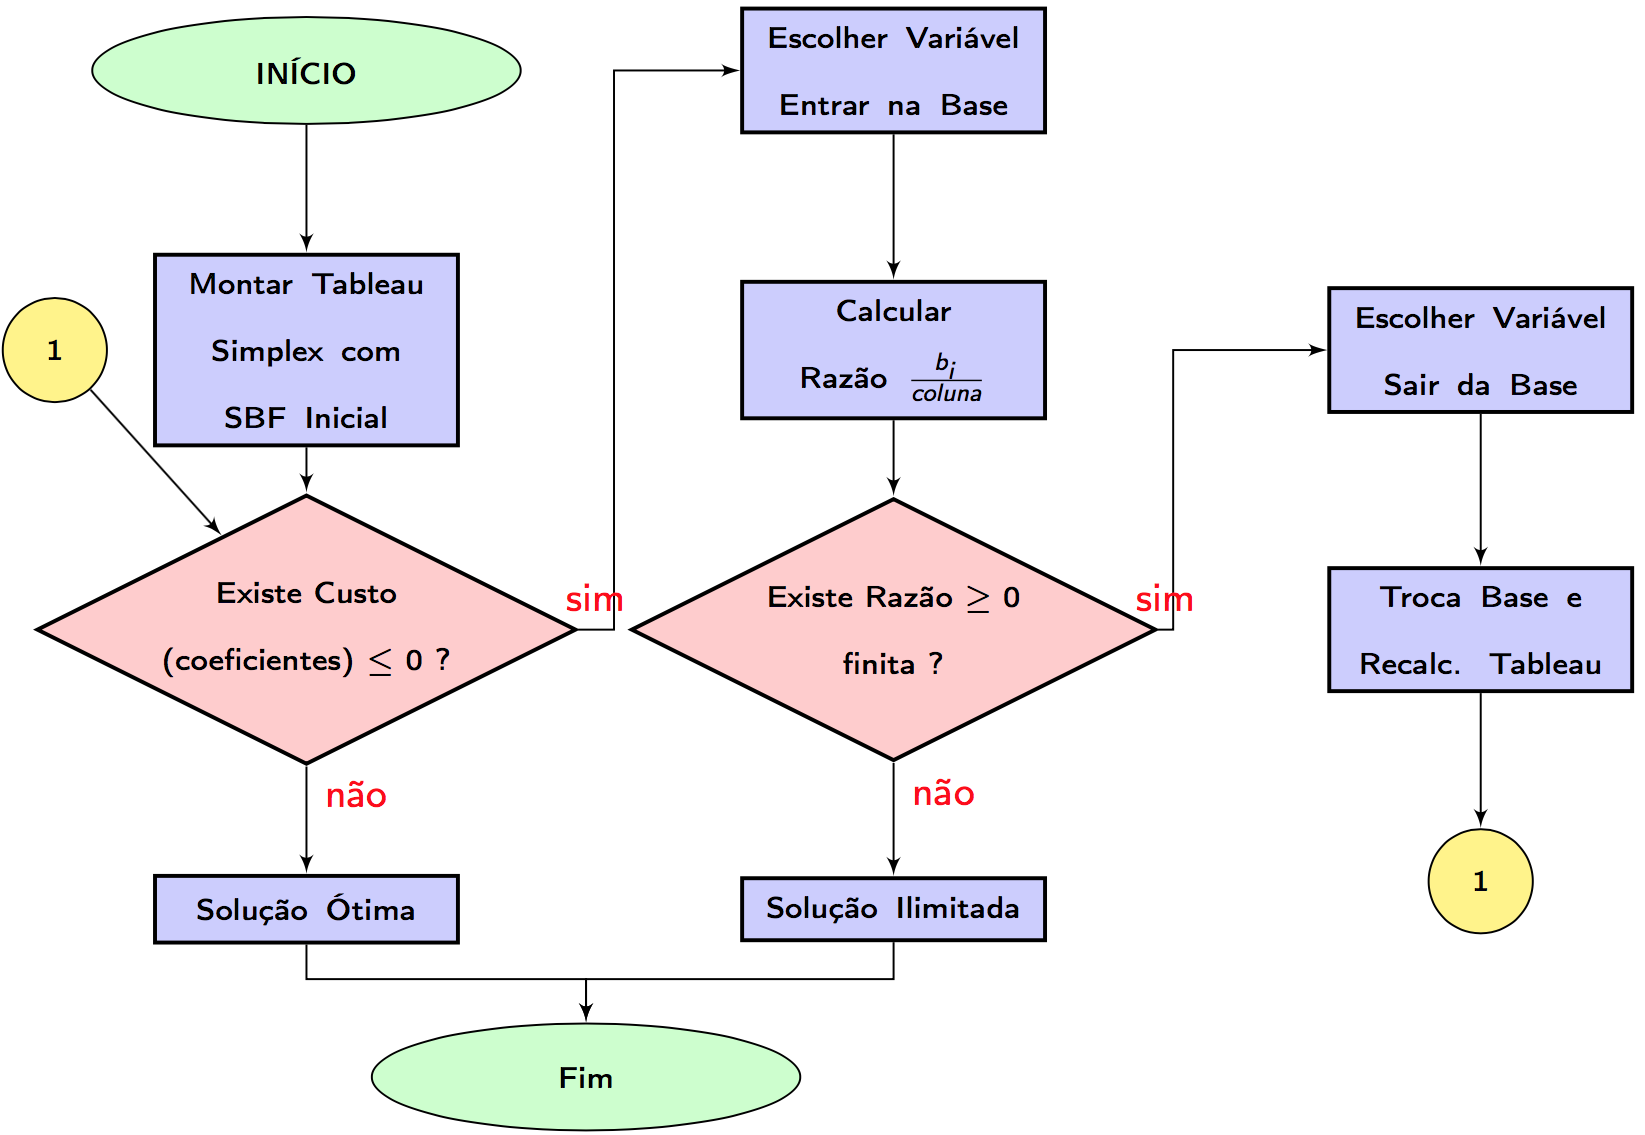
\includegraphics[width=5.5cm,height=3cm]{Alg_1.png}
			}
			\only<2>
			{
				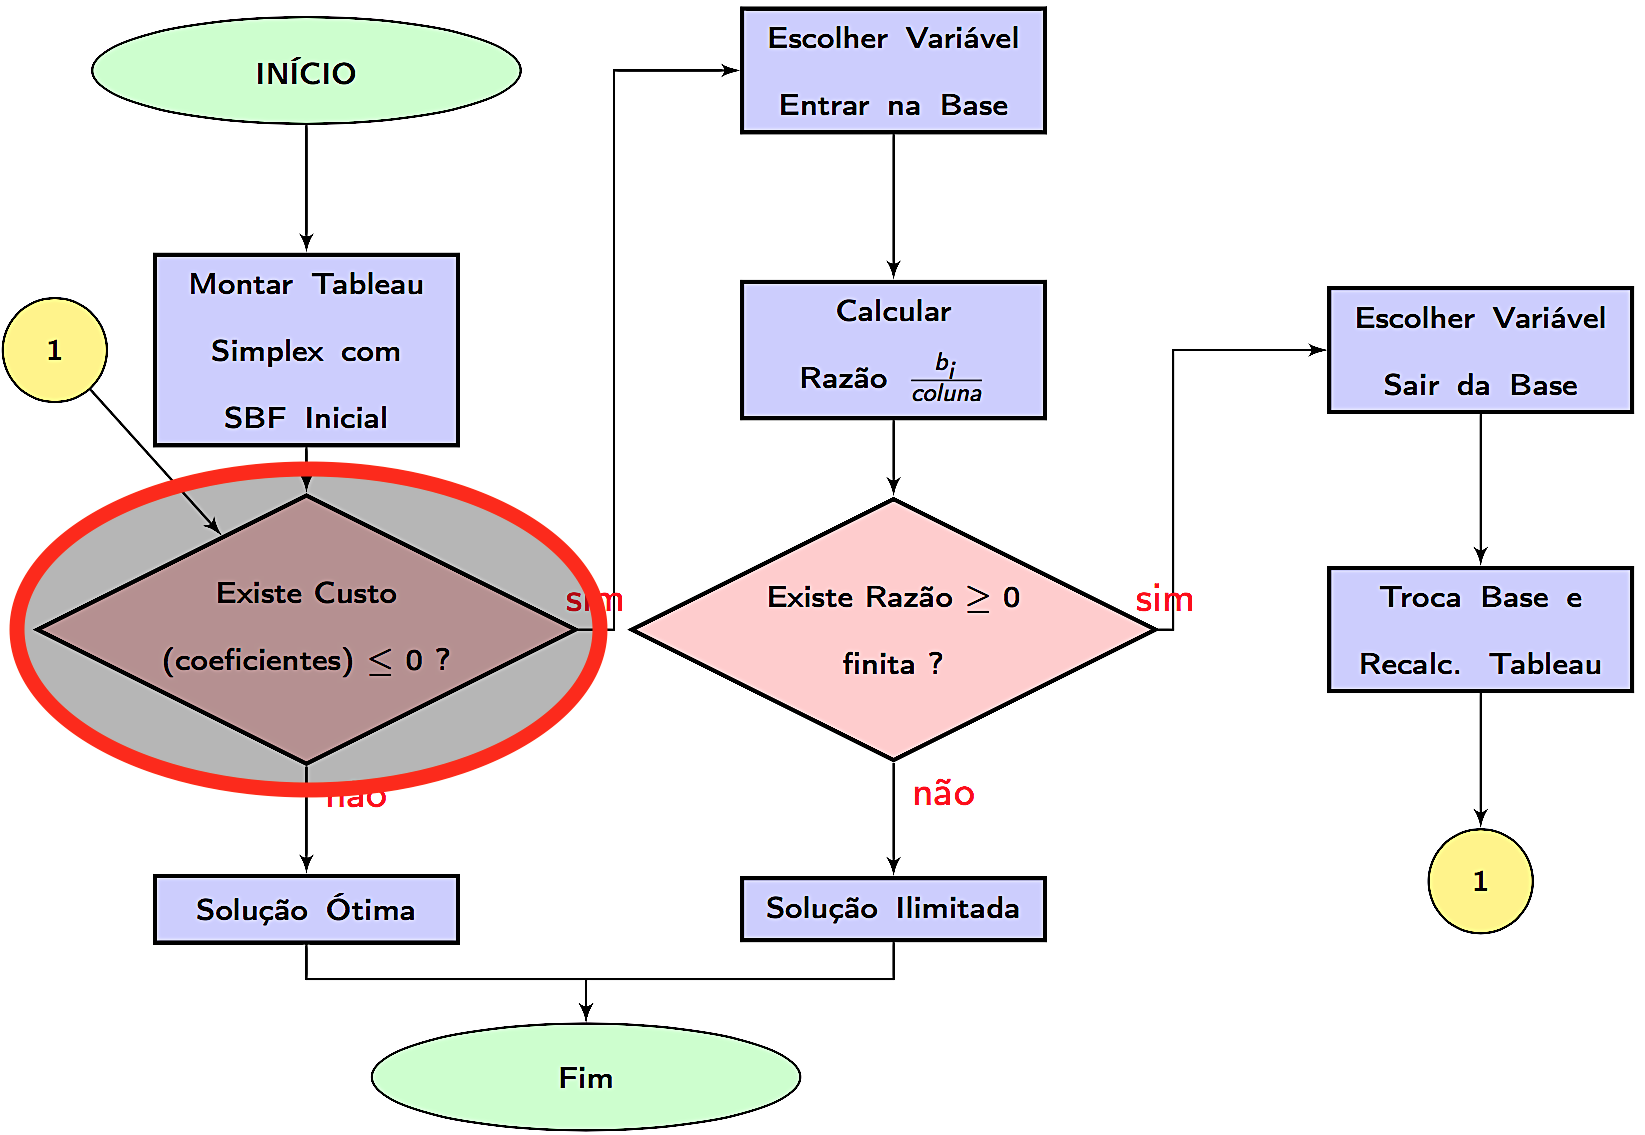
\includegraphics[width=5.5cm,height=3cm]{Alg_2.png}
			}
			\only<3>
			{
				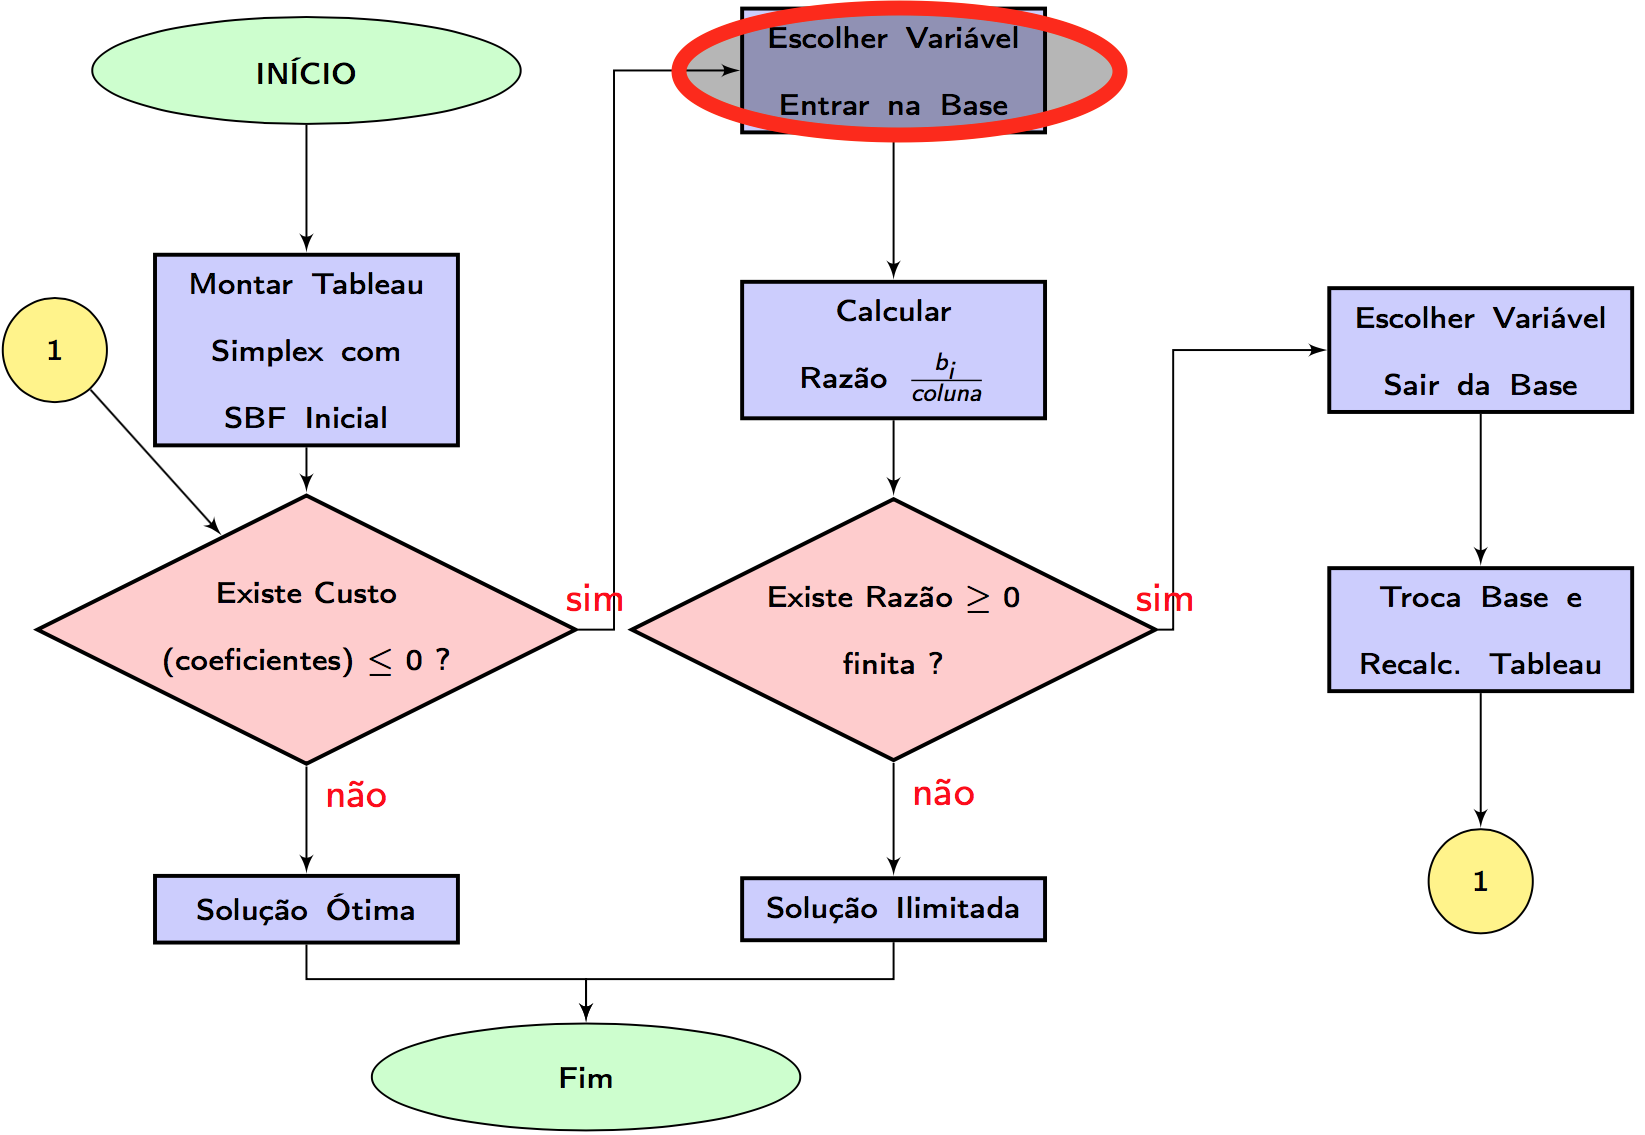
\includegraphics[width=5.5cm,height=3cm]{Alg_3.png}
			}
			\only<4>
			{
				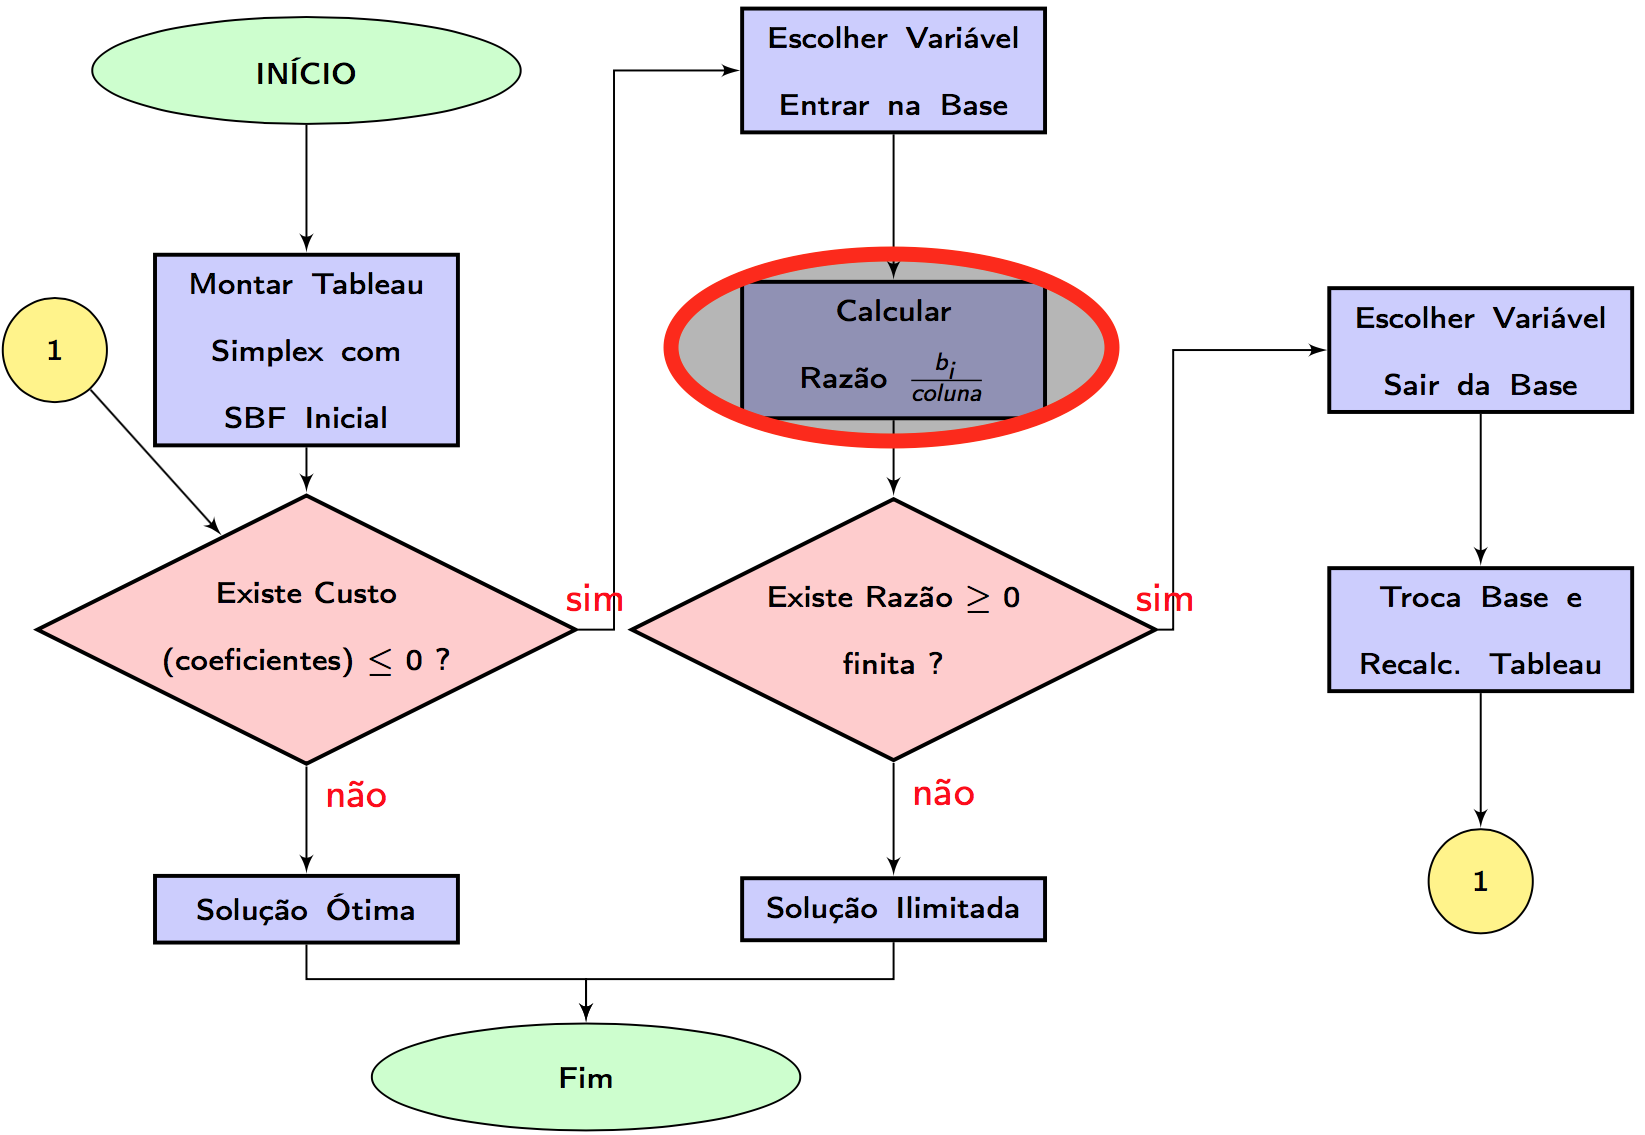
\includegraphics[width=5.5cm,height=3cm]{Alg_4.png}
			}
			\only<5>
			{
				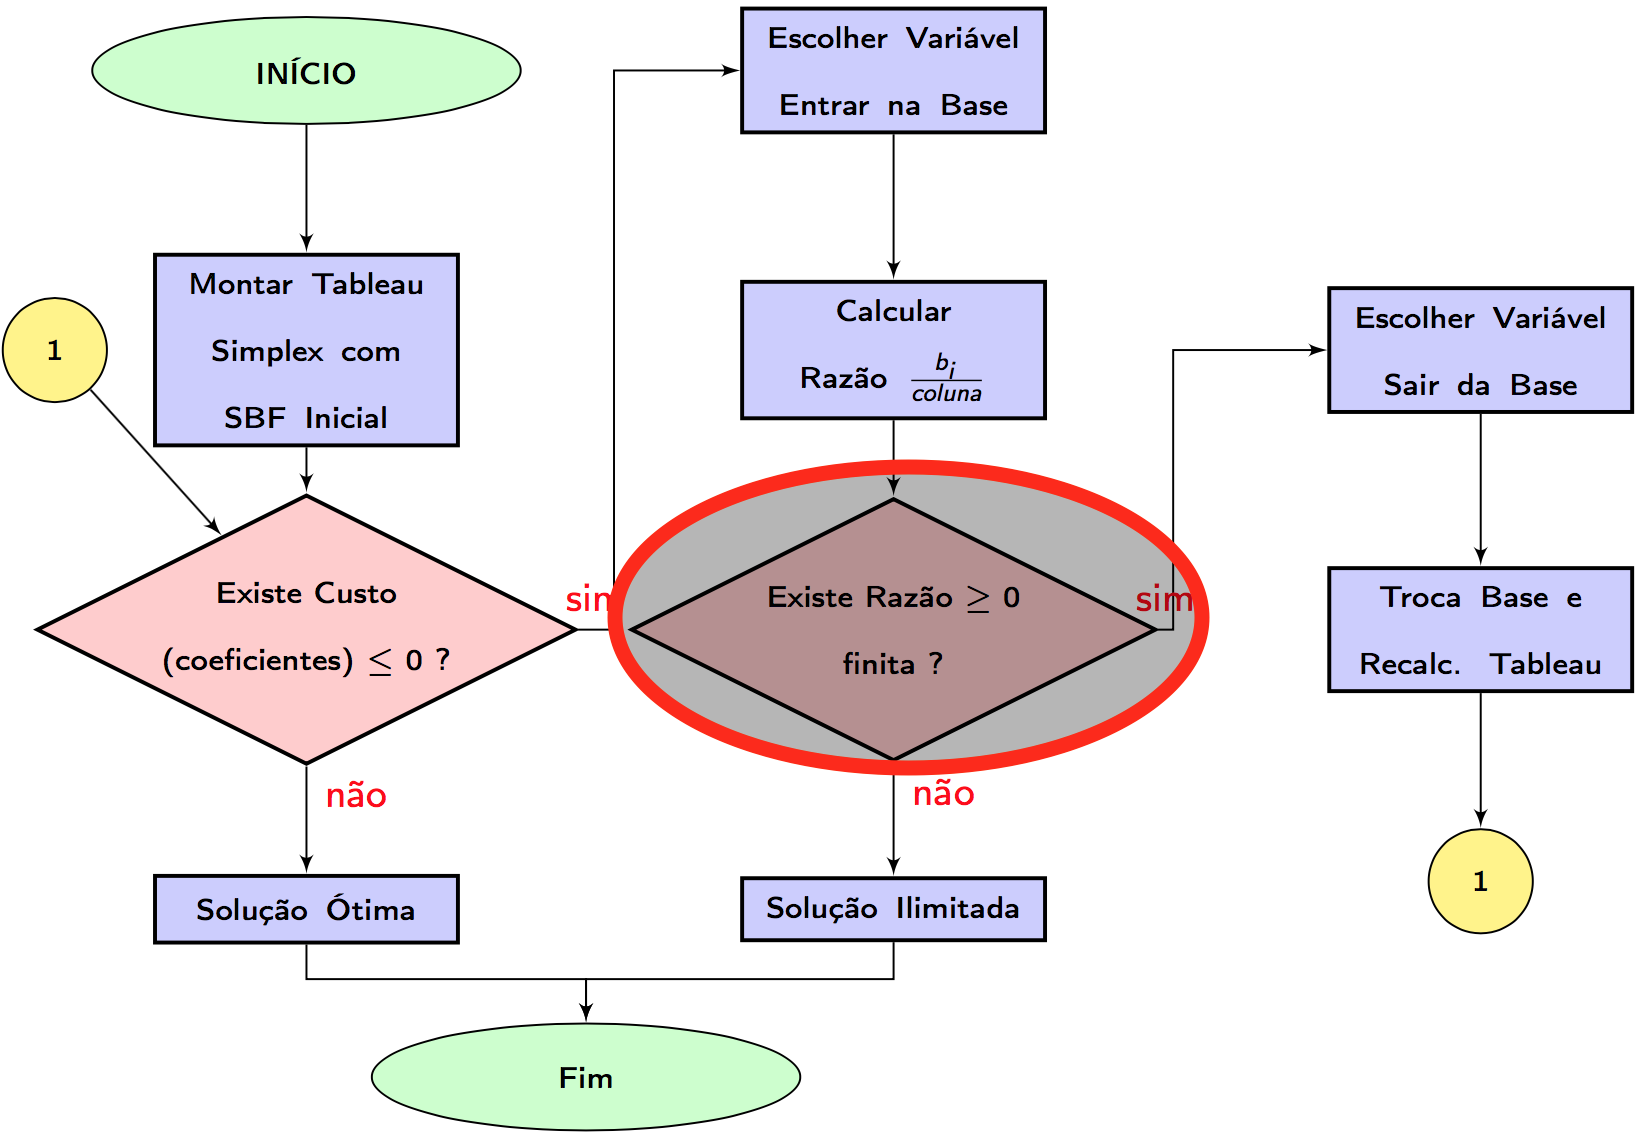
\includegraphics[width=5.5cm,height=3cm]{Alg_5.png}
			}
			\only<6>
			{
				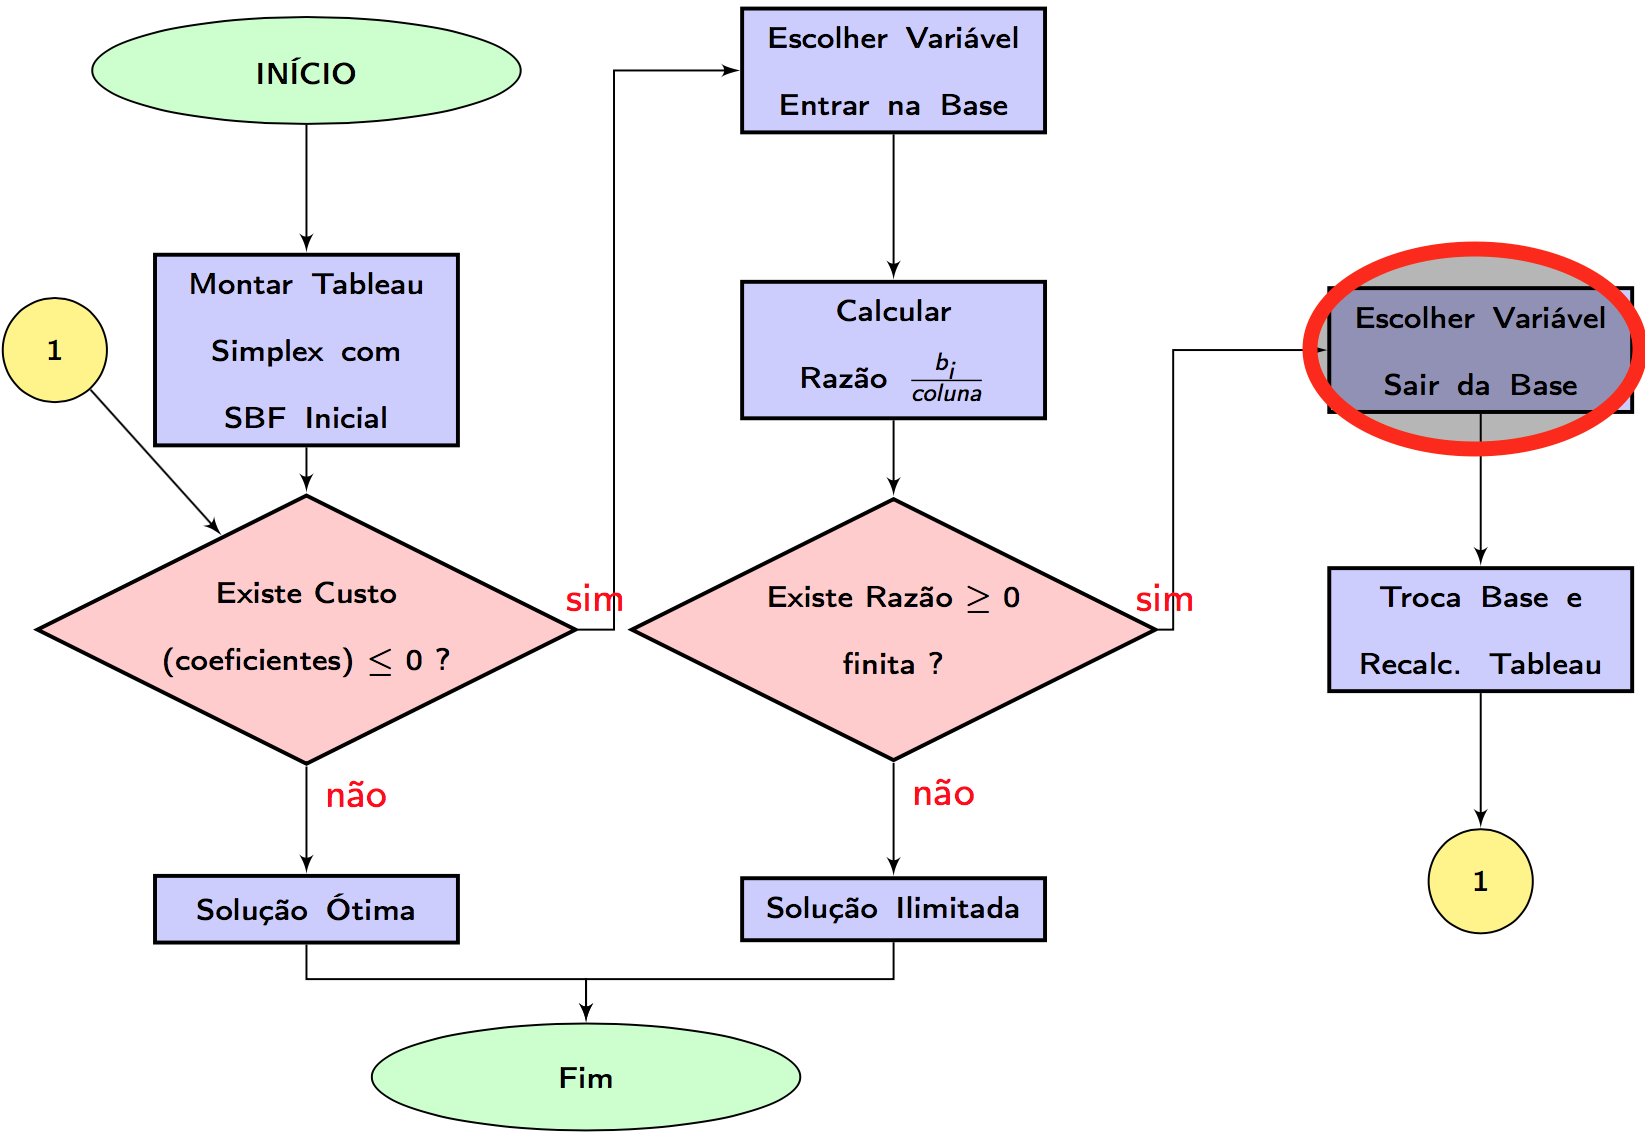
\includegraphics[width=5.5cm,height=3cm]{Alg_6.png}
			}
			\only<7-8>
			{
				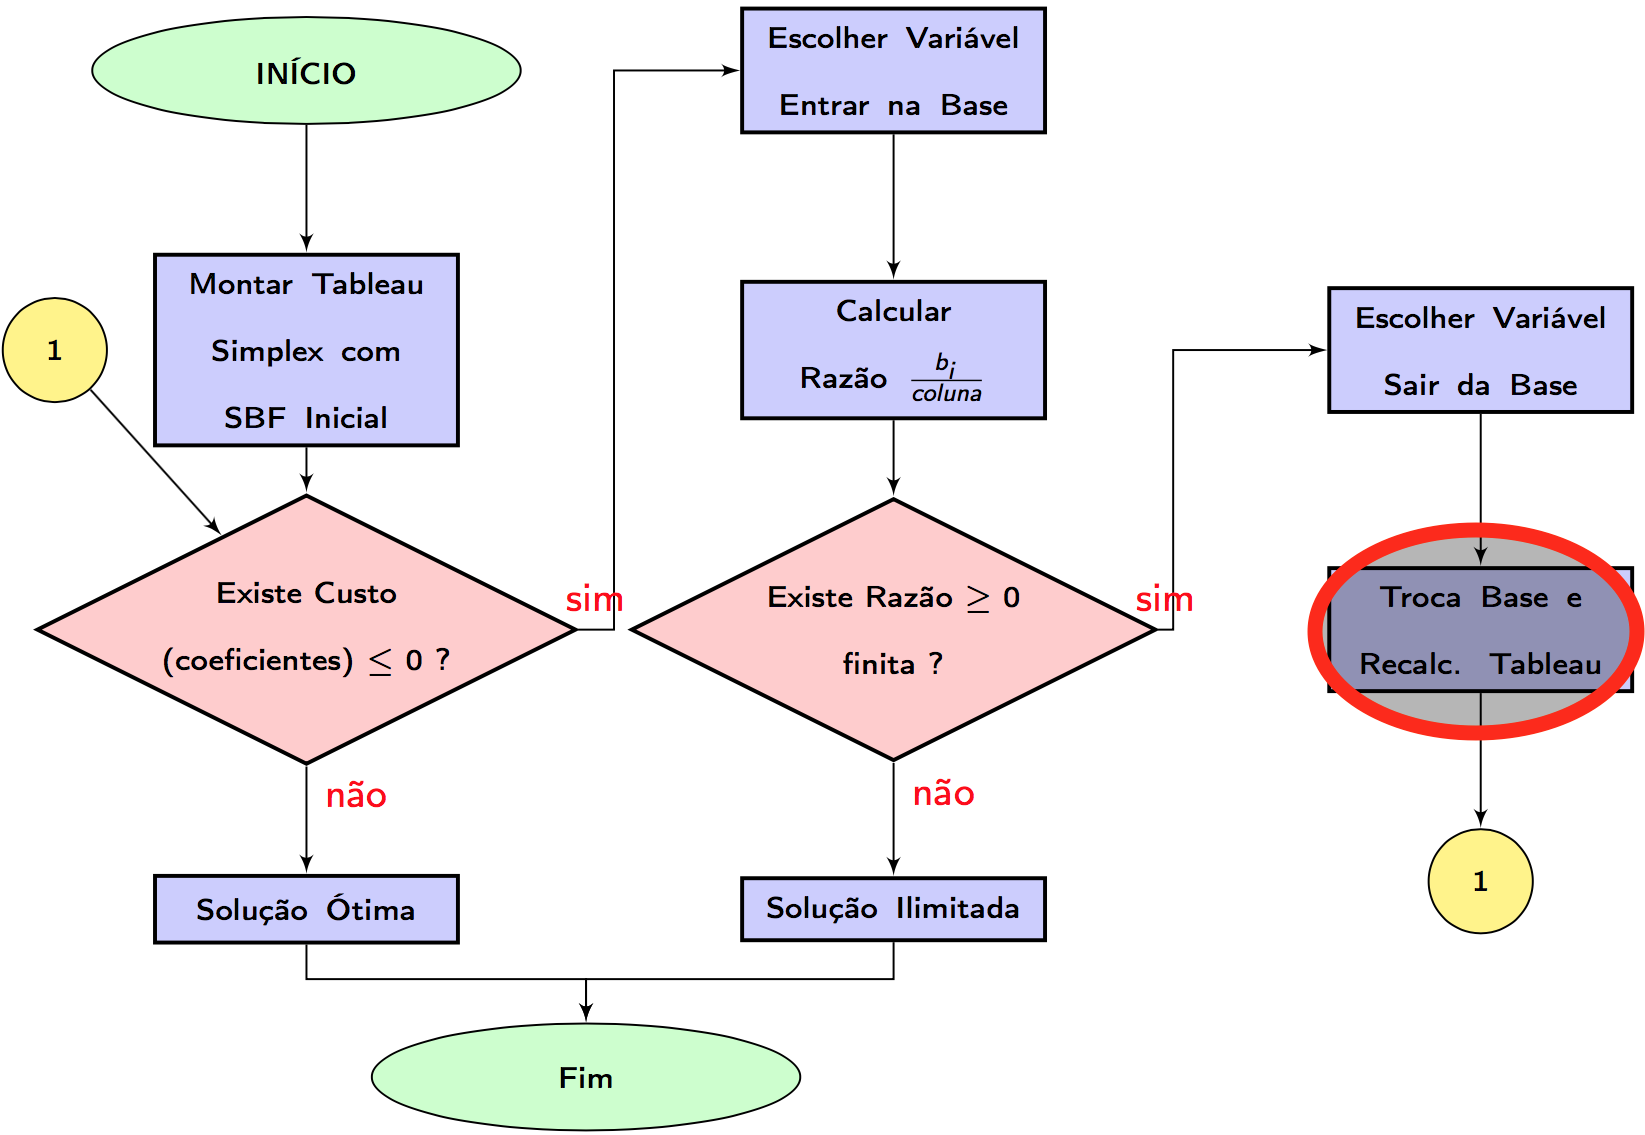
\includegraphics[width=5.5cm,height=3cm]{Alg_7.png}
			}
			\only<9>
			{
				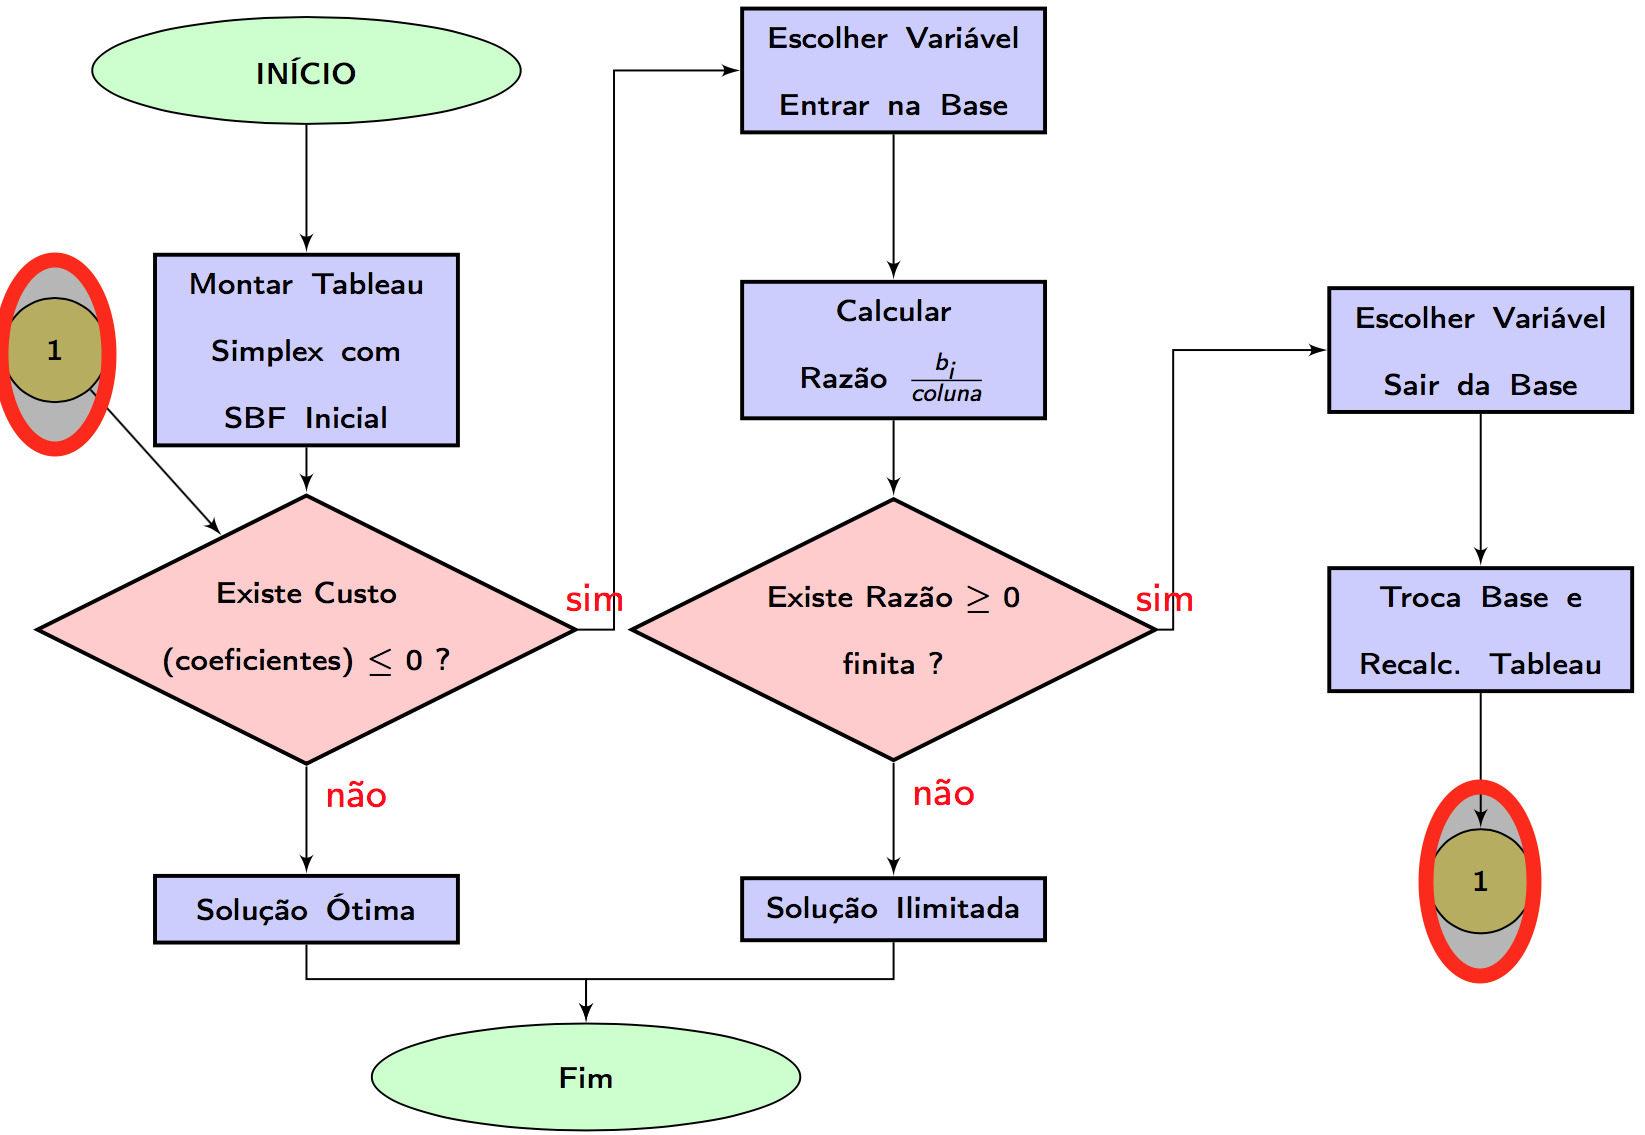
\includegraphics[width=5.5cm,height=3cm]{Alg_9.png}
			}
			\only<10>
			{
				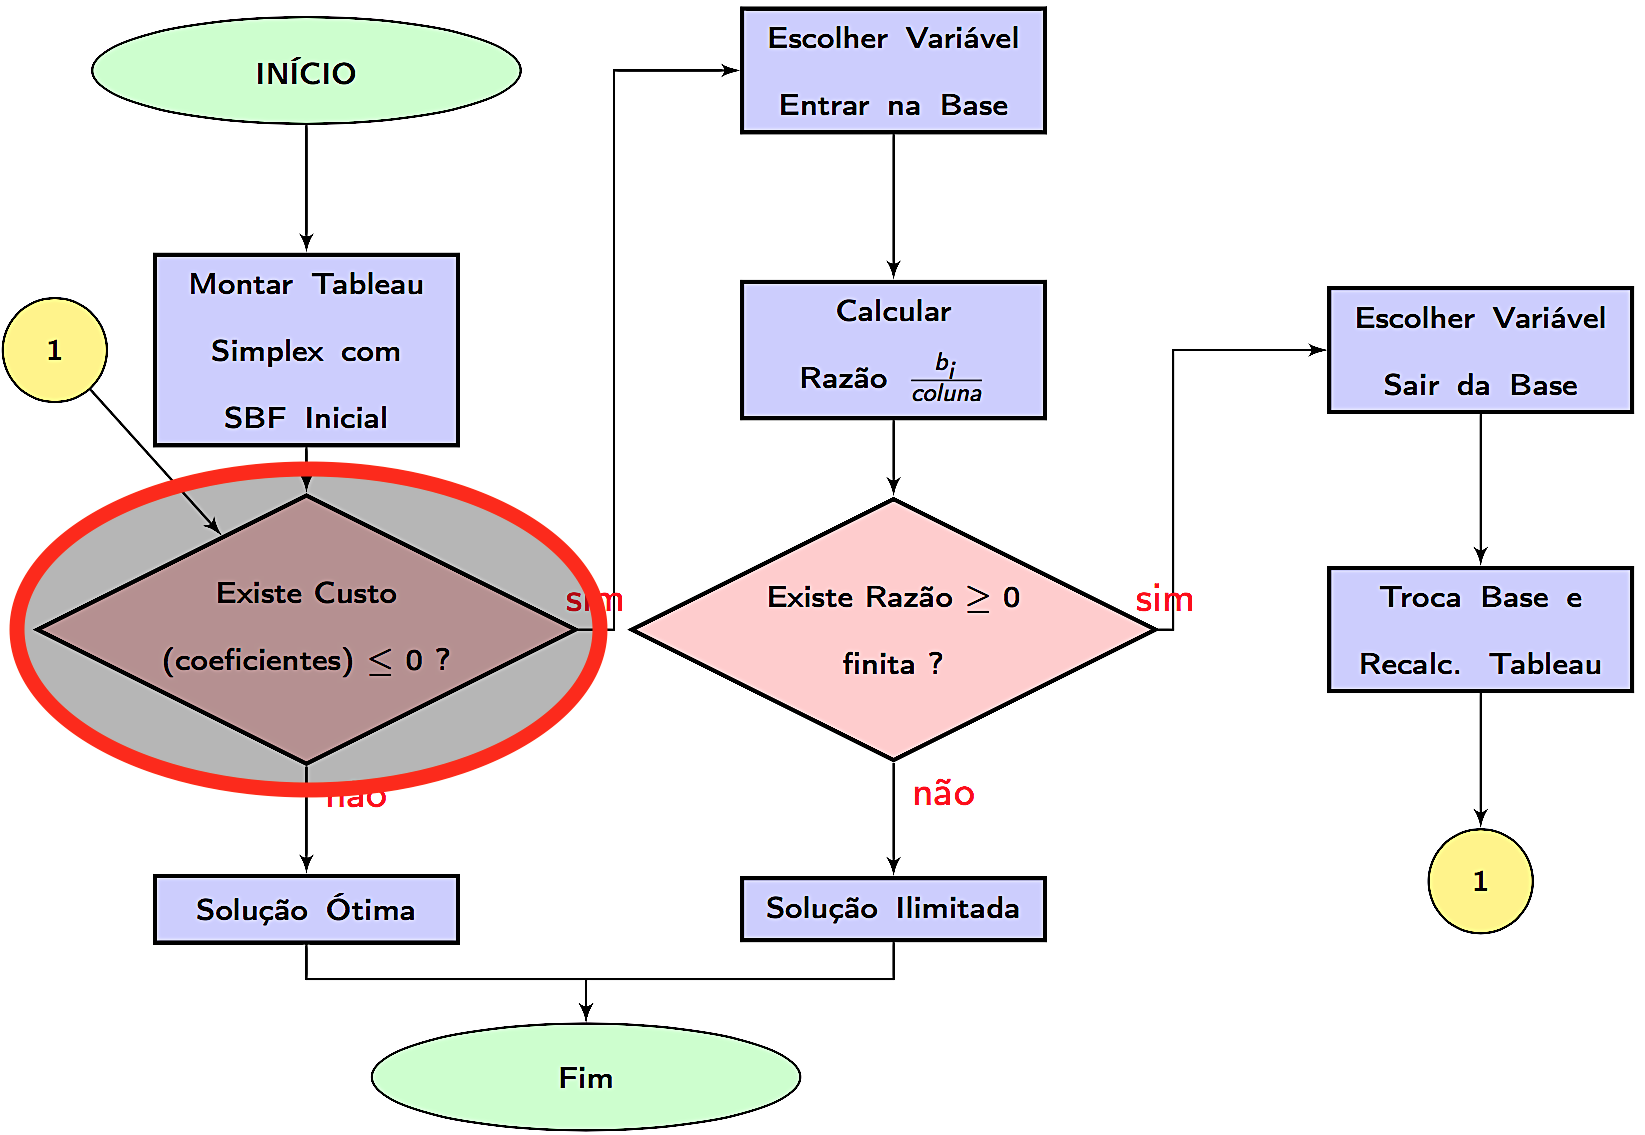
\includegraphics[width=5.5cm,height=3cm]{Alg_2.png}
			}
			\only<11>
			{
				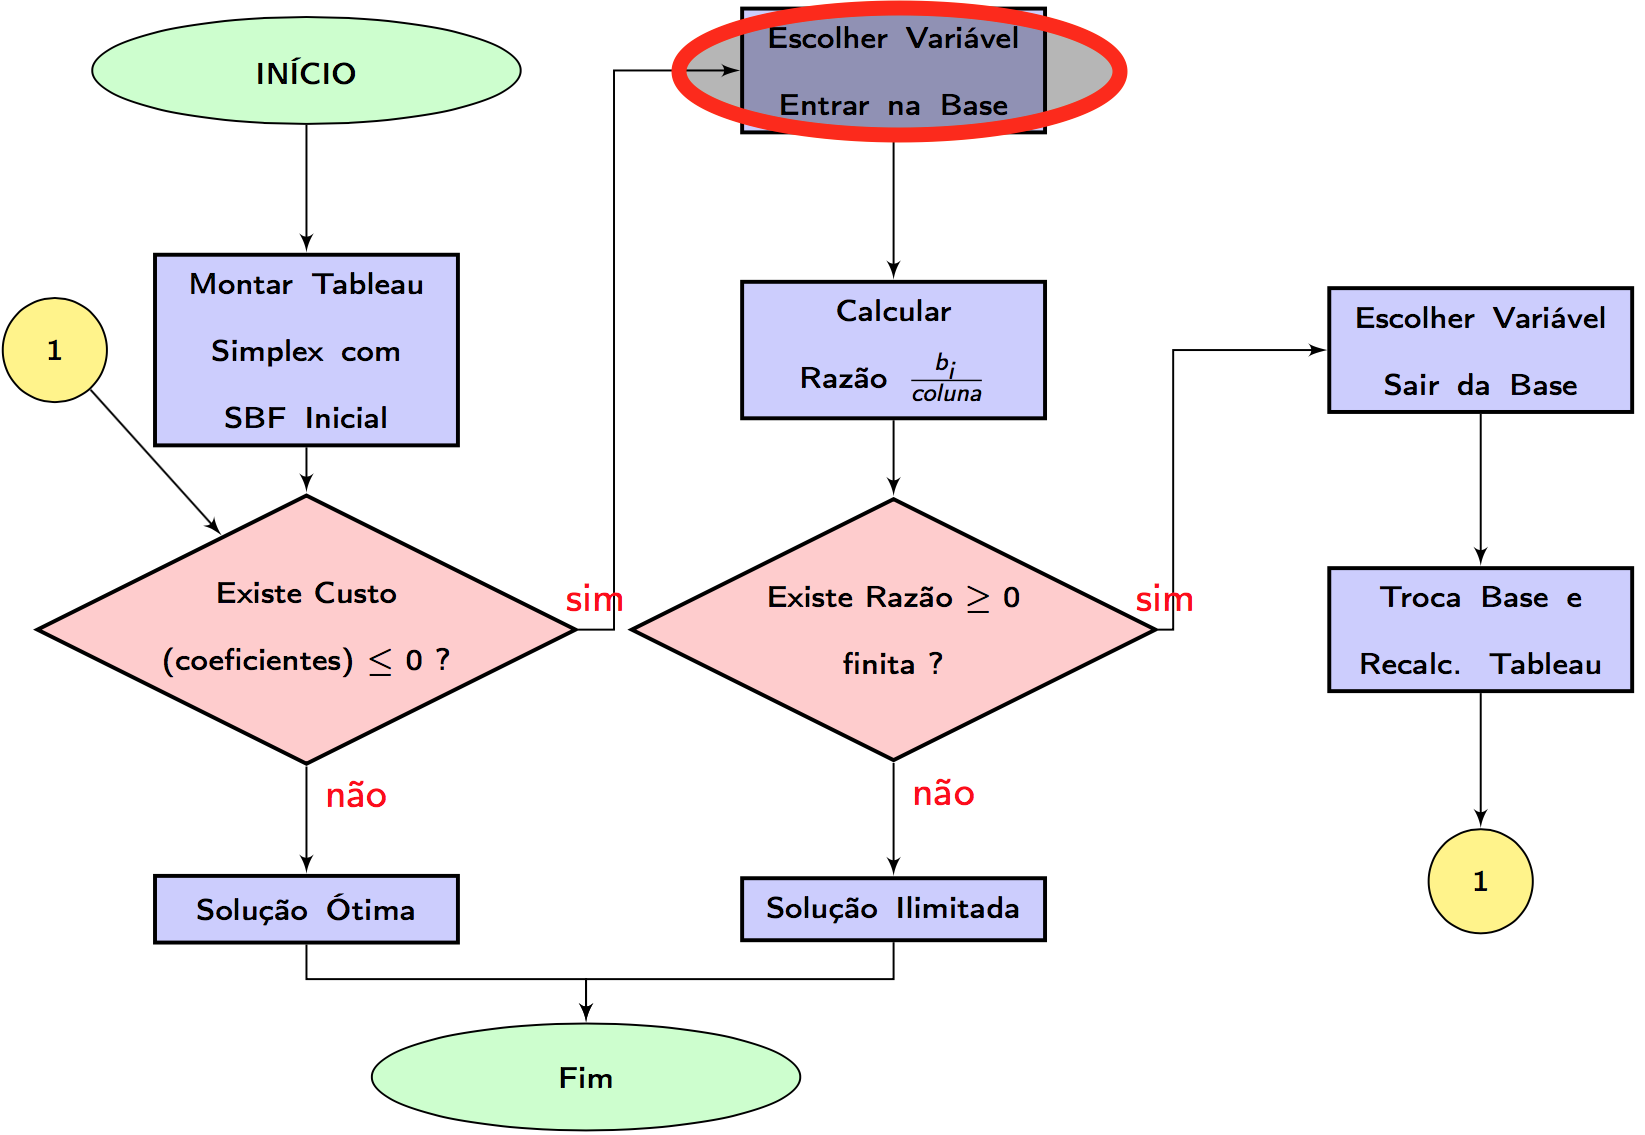
\includegraphics[width=5.5cm,height=3cm]{Alg_3.png}
			}
			\only<12>
			{
				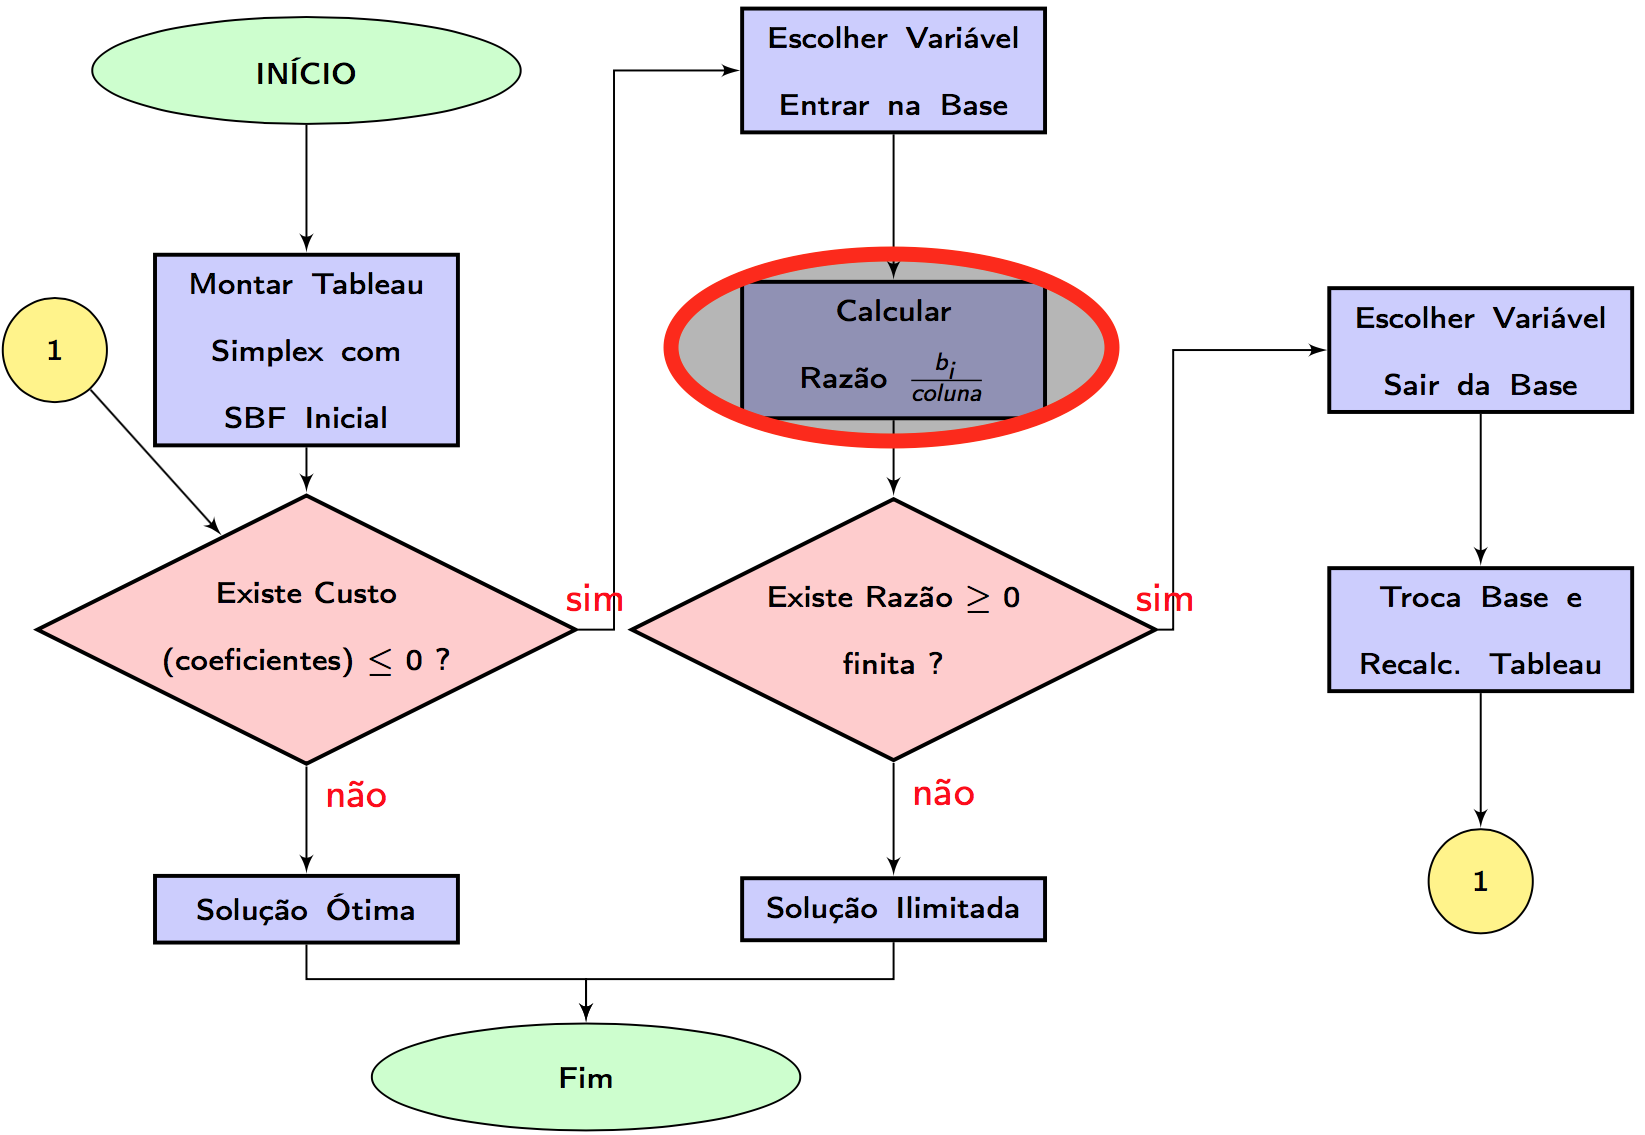
\includegraphics[width=5.5cm,height=3cm]{Alg_4.png}
			}
			\only<13>
			{
				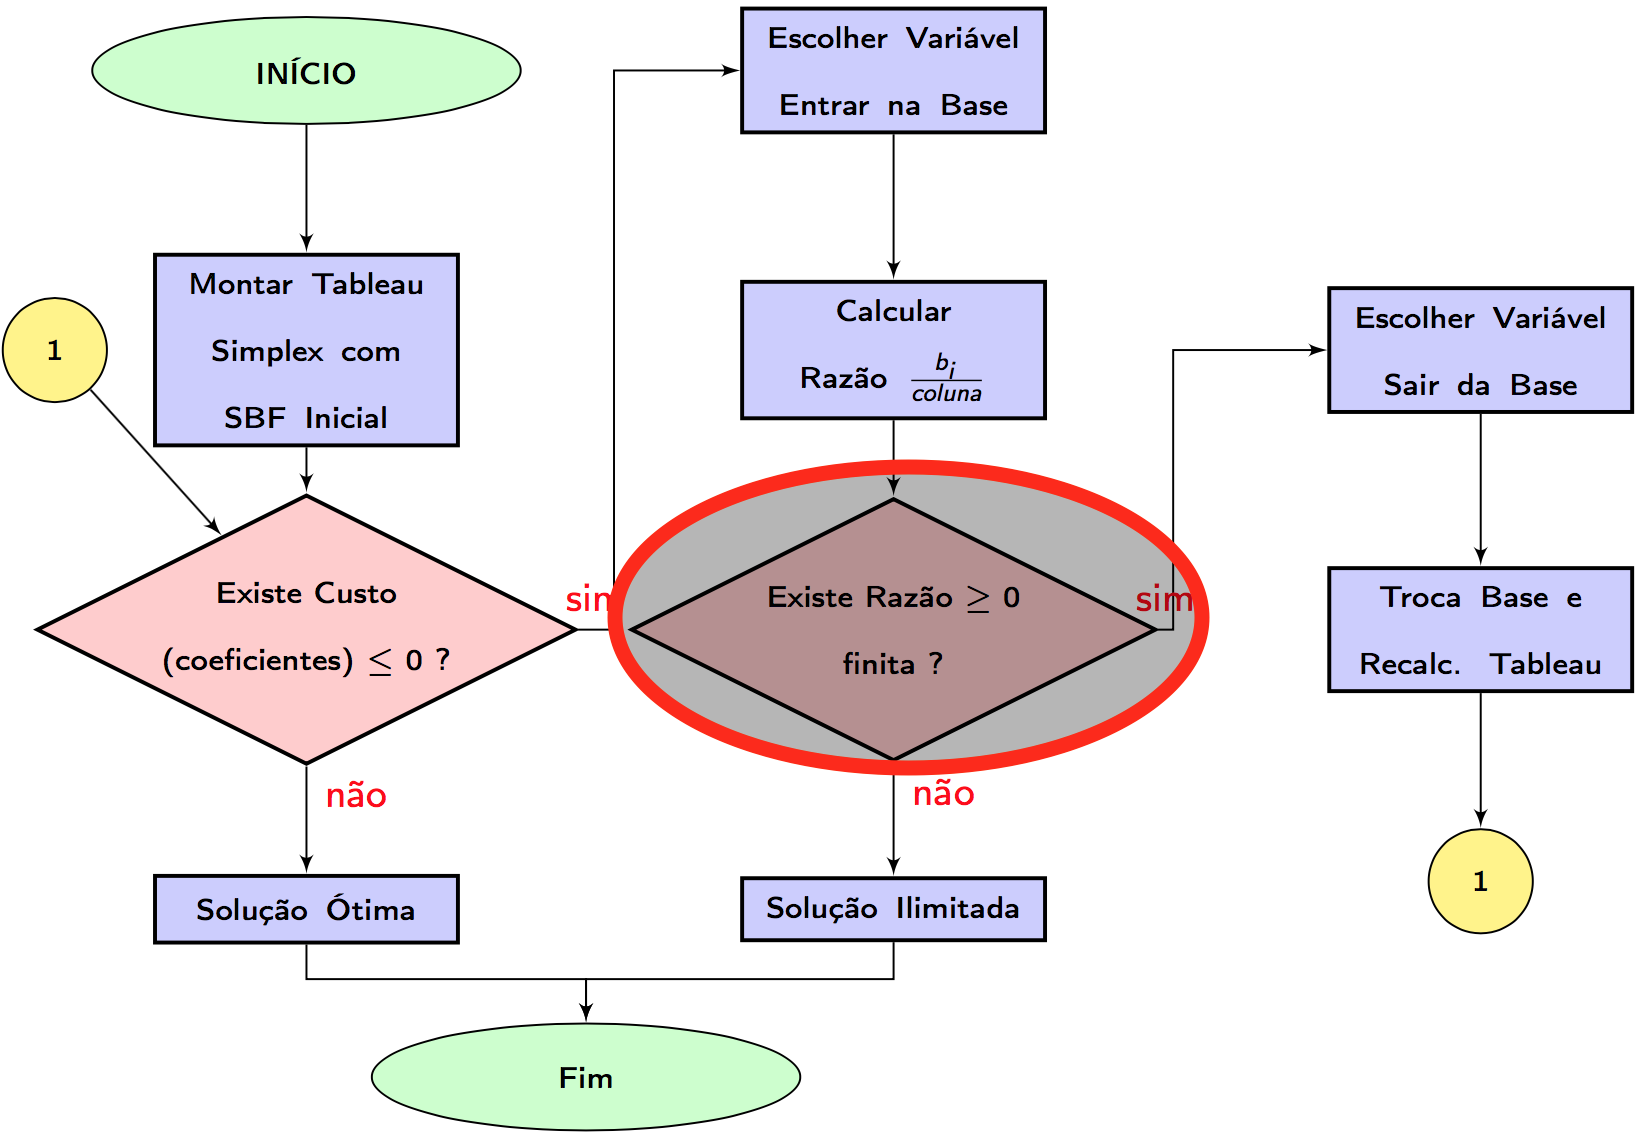
\includegraphics[width=5.5cm,height=3cm]{Alg_5.png}
			}
			\only<14>
			{
				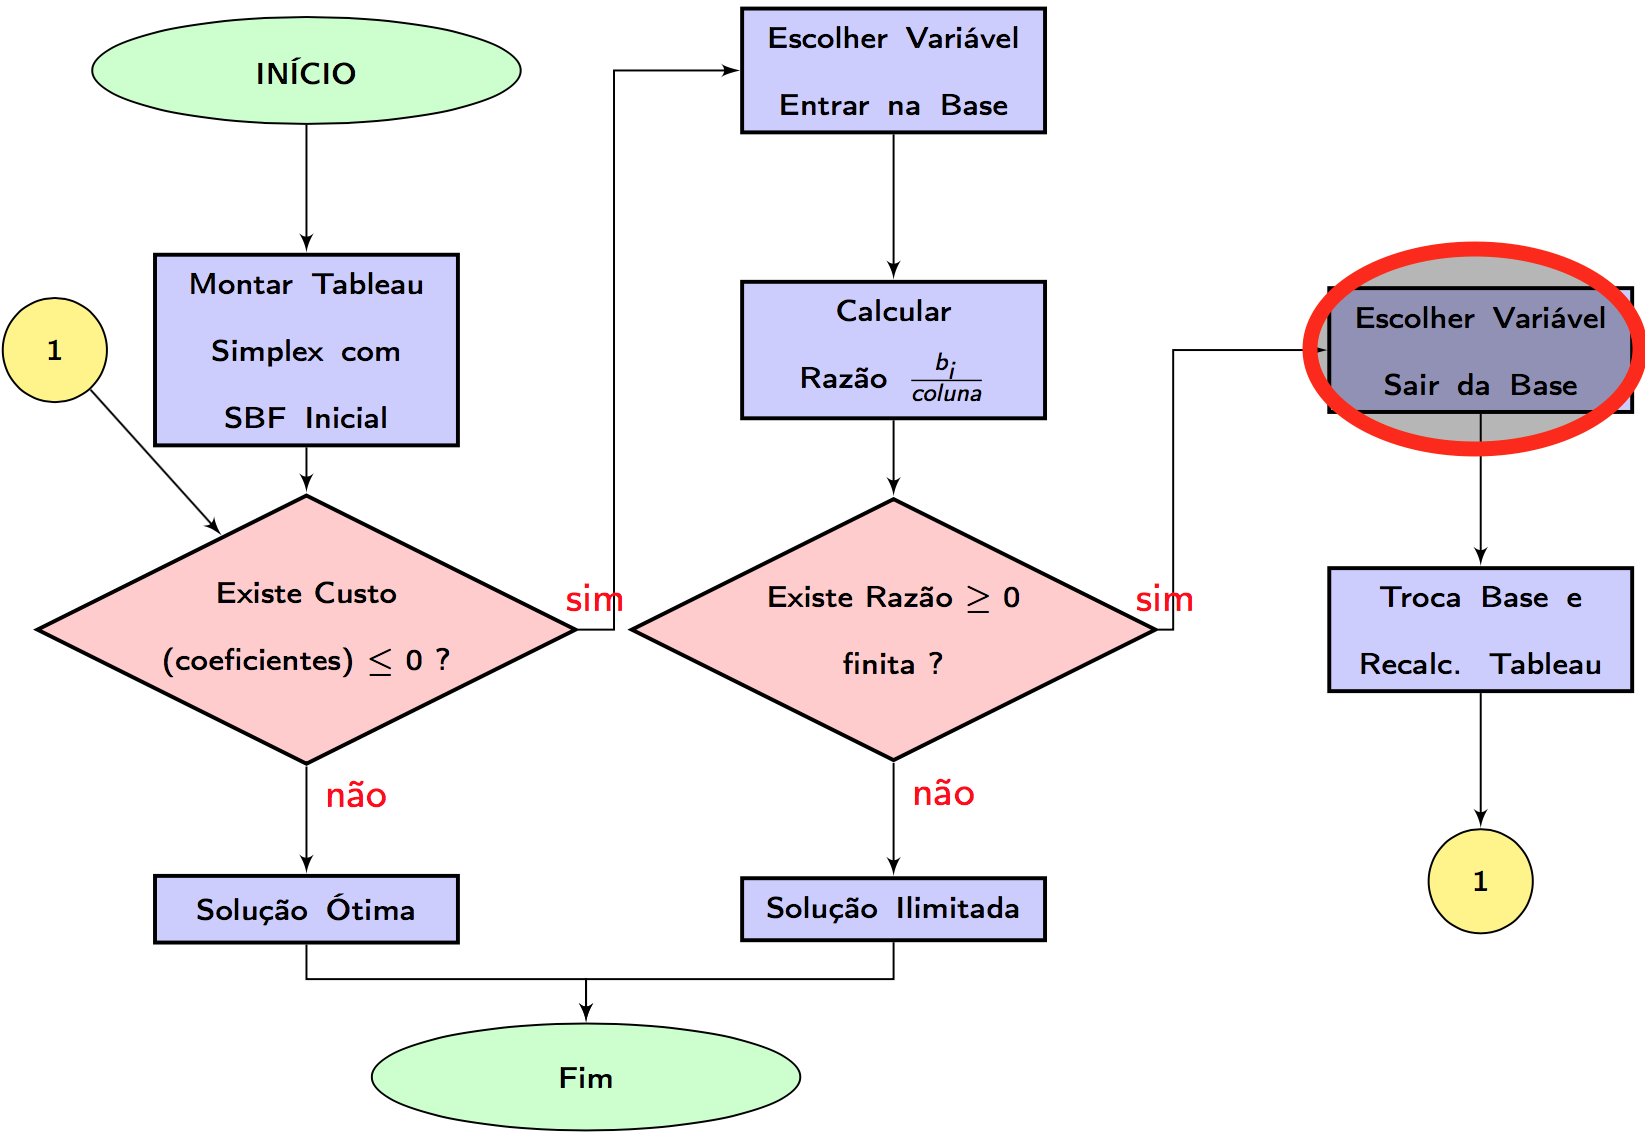
\includegraphics[width=5.5cm,height=3cm]{Alg_6.png}
			}
			\only<15-16>
			{
				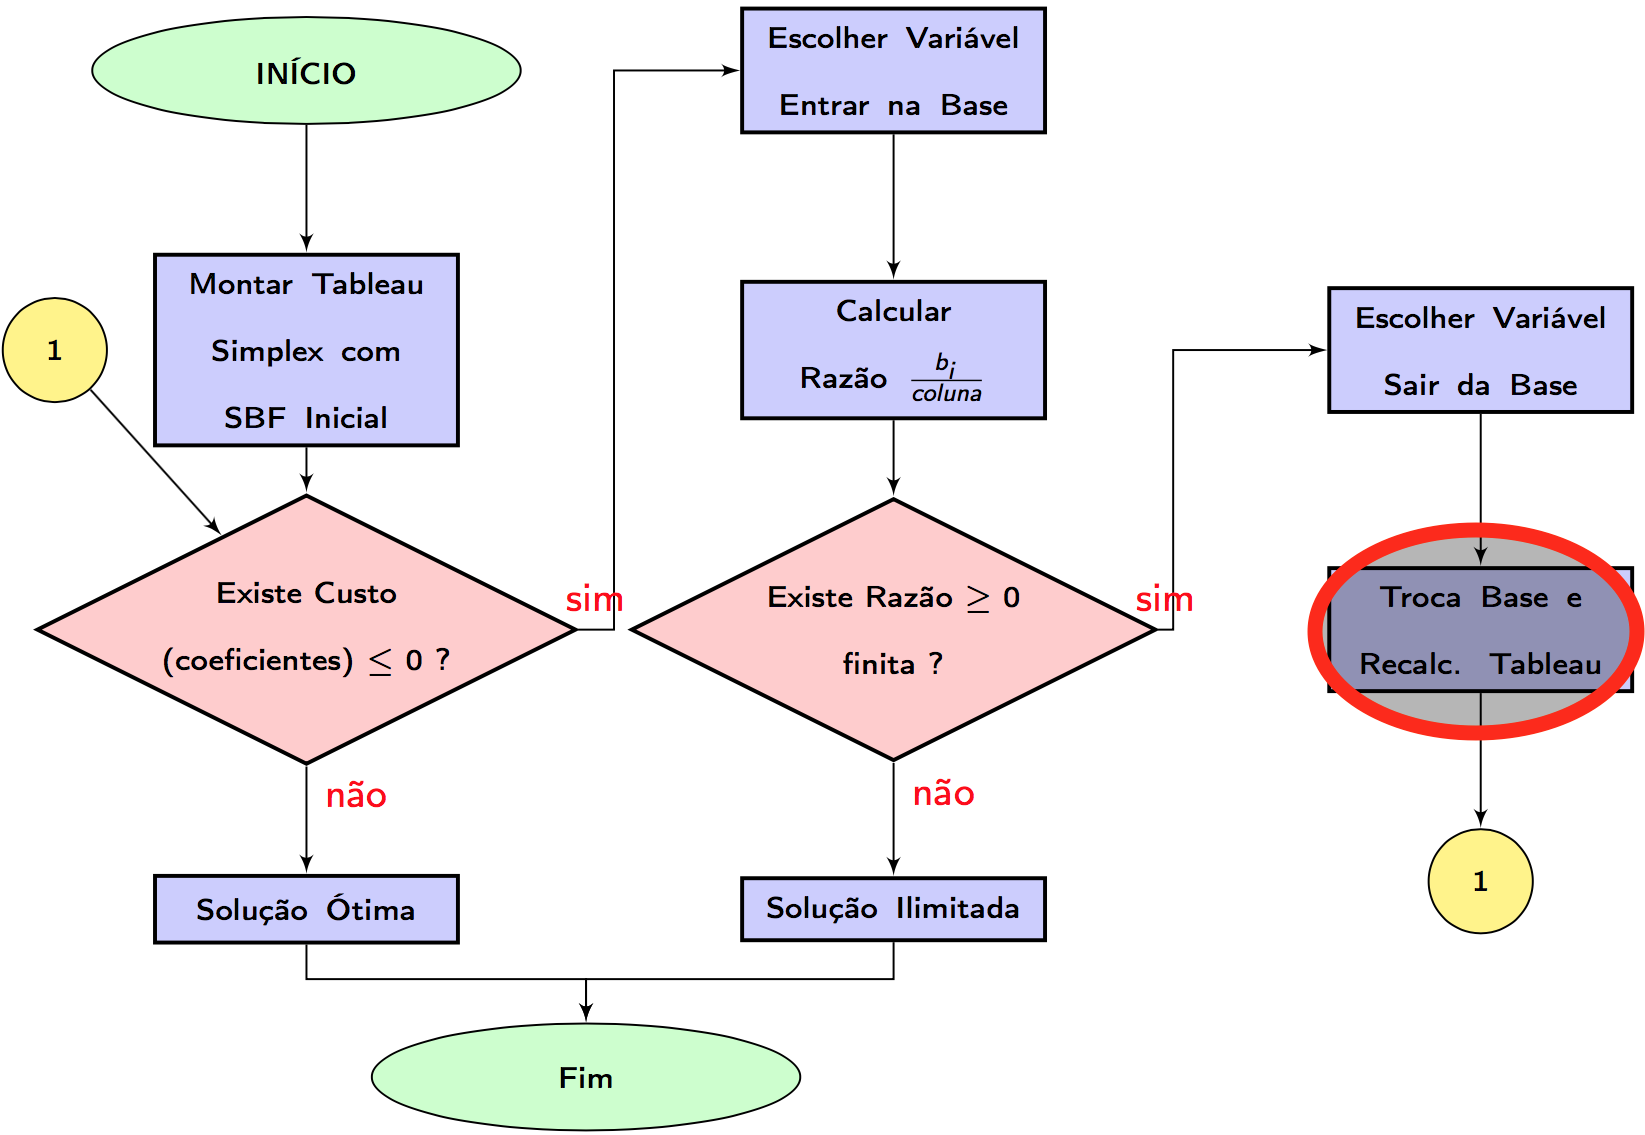
\includegraphics[width=5.5cm,height=3cm]{Alg_7.png}
			}
			\only<17>
			{
				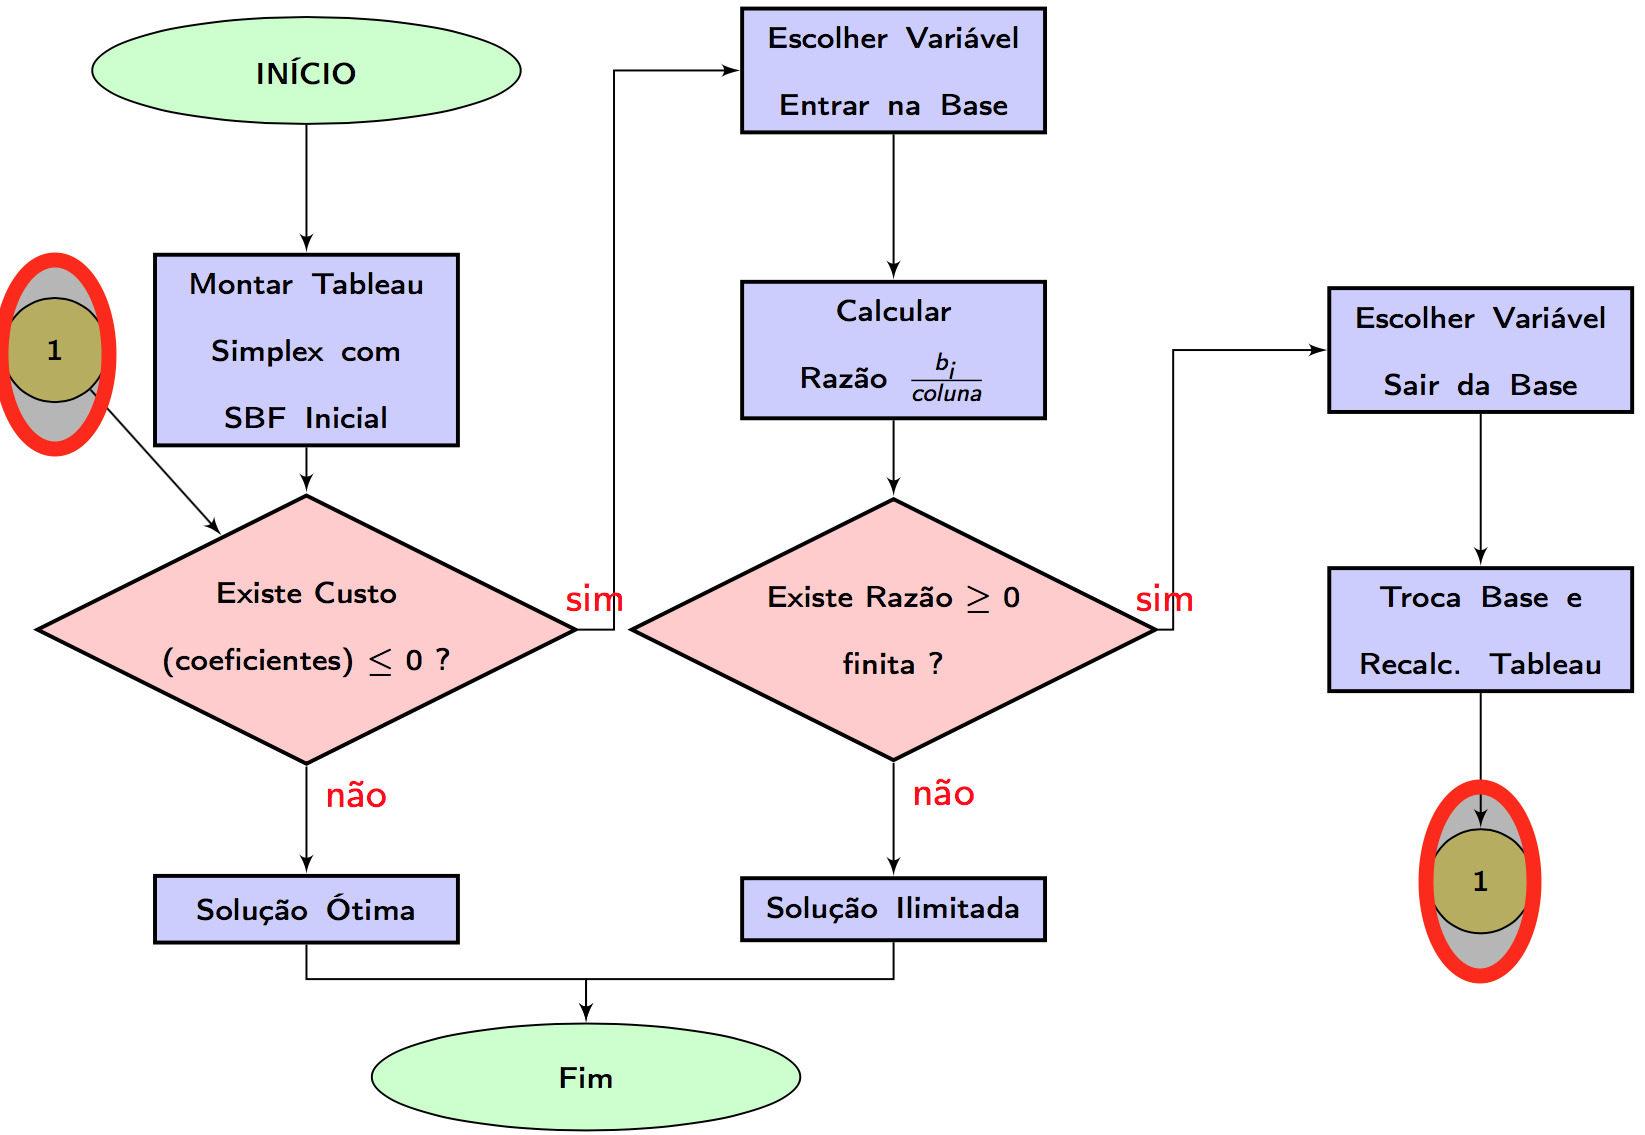
\includegraphics[width=5.5cm,height=3cm]{Alg_9.png}
			}
			\only<18>
			{
				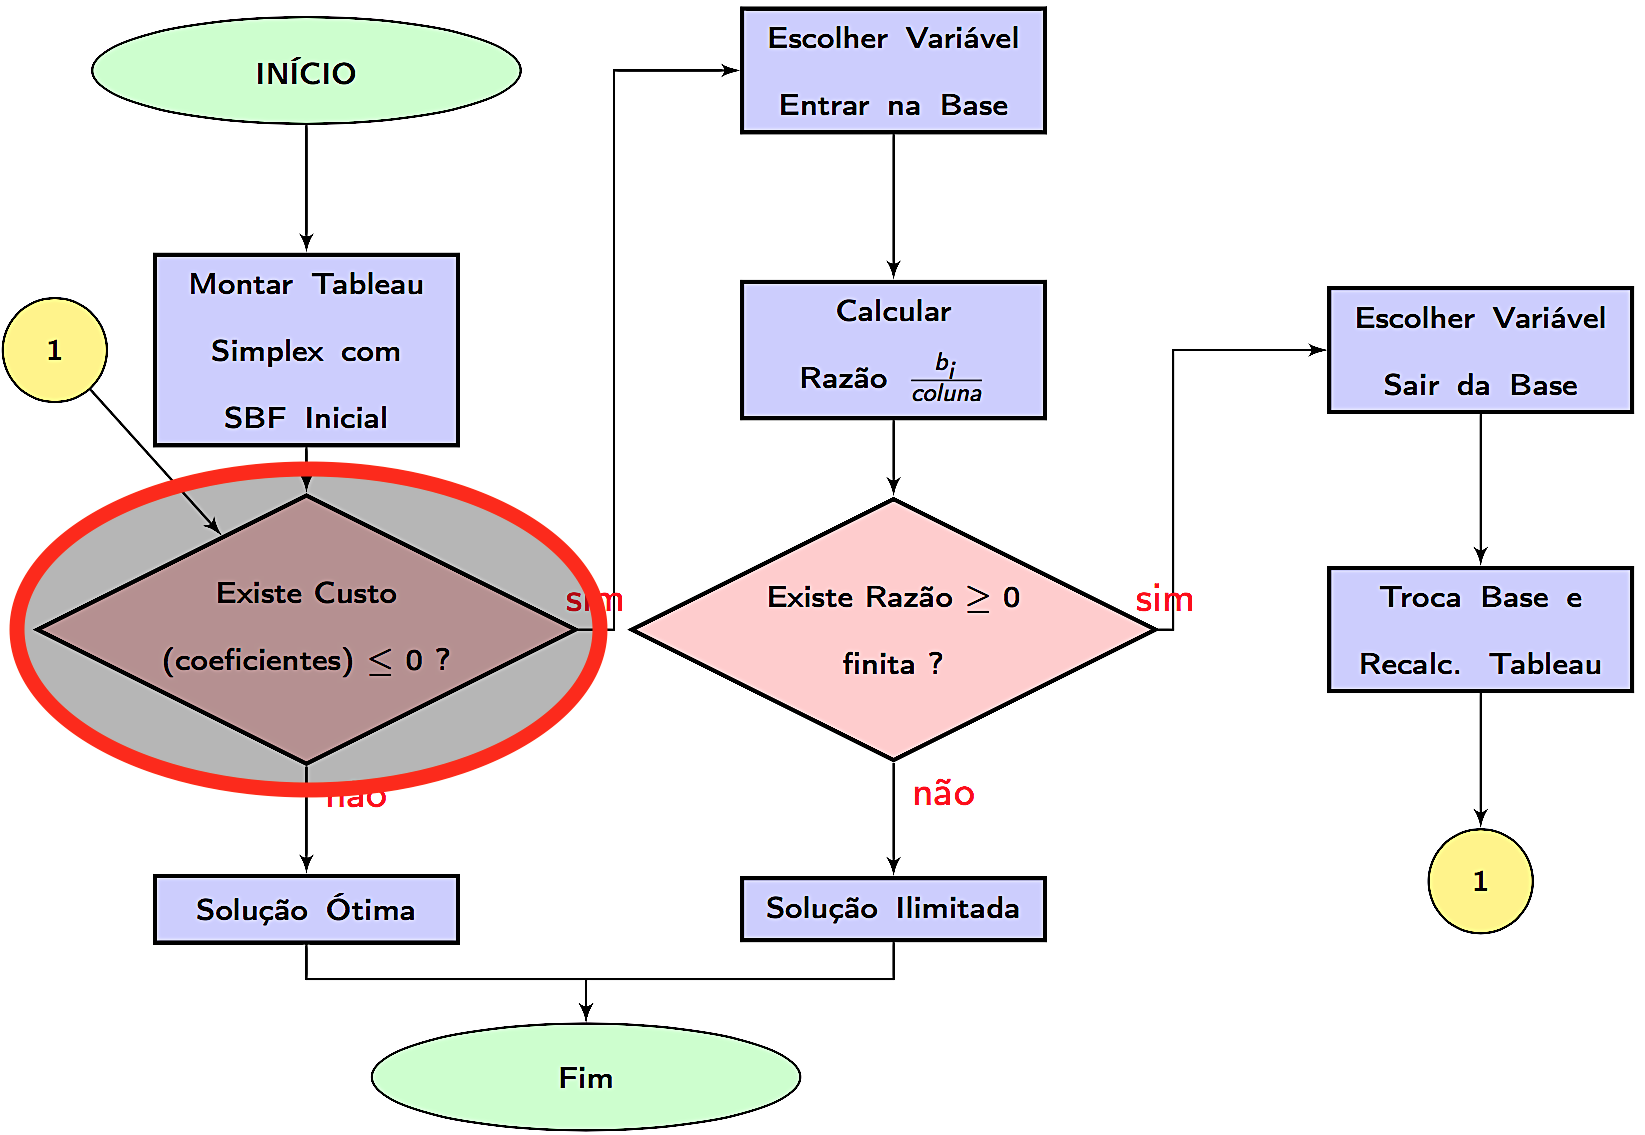
\includegraphics[width=5.5cm,height=3cm]{Alg_2.png}
			}
			\only<19-20>
			{
				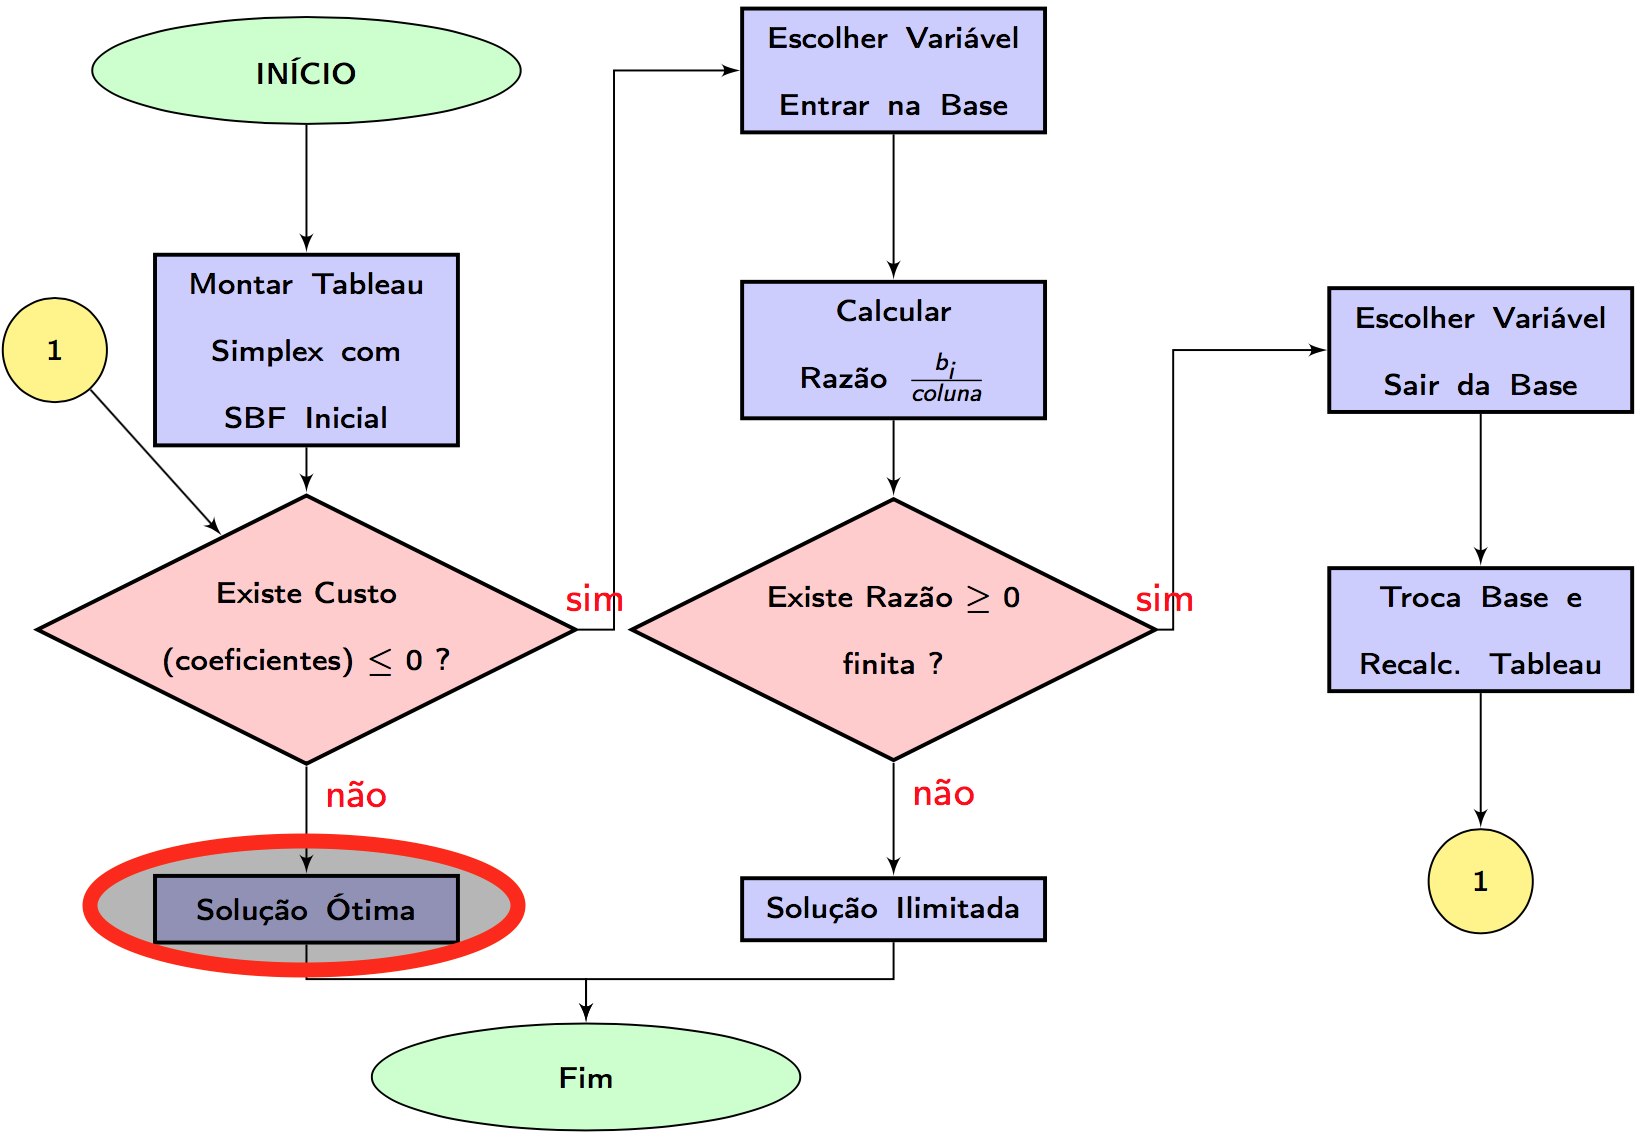
\includegraphics[width=5.5cm,height=3cm]{Alg_8.png}
			}
		\end{column}
	\end{columns}
\end{frame}


\subsection{Problema de Minimização}
\begin{frame}
	\only<1>
	{
		\frametitle{Fluxograma Tableau Simplex - \color{pink!100} MAXIMIZAÇÃO}
	}
	\only<2>
	{
		\frametitle{Fluxograma Tableau Simplex - \color{cyan!100} MINIMIZAÇÃO}
	}


	\centering
	\only<1>
	{
	\begin{tikzpicture} [
							auto, node distance = 2cm,
							decisao/.style = { diamond, draw, shape aspect=2, thick, fill=red!20,
							                   text width=6em, text badly centered,
							                   inner sep=1pt},
							bloco/.style   = { rectangle, draw, thick, fill=blue!20, 
												text width=5em, text centered,
							                   minimum height=1em },
							bloco2/.style   = { rectangle, draw, thick, fill=blue!20, 
												text width=5em, text centered,
							                   minimum height=1em, node distance = 4.2cm },
							extremo/.style  = { ellipse, draw, fill=green!20,
							                   text width=5em, text centered,
							                   minimum height=2em },	
							line/.style   = { draw, -latex' },
							goto/.style = {circle, draw, fill=yellow!60, text width=1em,
										   text centered, node distance = 1.8cm},
						    bullet/.style = {rectangle, draw, thick, fill=red!80, 
						    				text width=9em, text centered,
						    				minimum height=1em},
						]

	
		\node [extremo] (inic) {\tiny INÍCIO}; 
		
		\node [bloco, below of = inic] (sbfi) {\tiny Montar Tableau Simplex com SBF Inicial};
		\path [line] (inic) -- (sbfi); 
		
		\node [decisao, below of = sbfi] (conv) {\tiny Existe Custo (coeficientes) $<$ 0 ?} ;
		\path [line] (sbfi) -- (conv); 
		
		\node[bloco, below of = conv] (otimo) {\tiny Solução Ótima};
		\path [line] (conv) -- node [near start] {\scriptsize \color{red} não} (otimo); 
	    \node [extremo] at (2,-7.2) (fim) {\tiny Fim};	
	    \path [line] (otimo) |- (2,-6.5) -- (fim); 

		\node[bloco2, right of = inic] (escolhe) {\tiny Escolher Variável Entrar na Base};
		\path [line] (conv) -| (2.2, 0) node [near start] {\scriptsize \color{red} sim} -- (escolhe); 
		
		\node[bloco, below of = escolhe] (razao) {\tiny Calcular Razão $ \frac{b_i}{coluna}$};
		\path [line] (escolhe) -- (razao); 

		\node [decisao, below of = razao] (finito) {\tiny Existe Razão $\ge 0$ finita ?} ;
		\path [line] (razao) -- (finito); 
		
		\node[bloco, below of = finito] (ilimit) {\tiny Solução Ilimitada};
		\path [line] (finito) -- node [near start] {\scriptsize \color{red} não} (ilimit); 
		\path [line] (ilimit) |- (2,-6.5) -- (fim); 

		\node[bloco2, right of = razao] (saibase) {\tiny Escolher Variável Sair da Base};
		\path [line] (finito) -| (6.2, -2) node [near start] {\scriptsize \color{red} sim} -- (saibase);
		
		\node[bloco, below of = saibase] (swap) {\tiny Troca Base e Recalc. Tableau};
		\path[line] (saibase) -- (swap); 
		
		\node[goto, below of = swap] (pula_a) {\tiny 1};
		\node[goto, left of = sbfi] (pula_b) {\tiny 1};
		\path[line] (pula_b) -- (conv);
		\path[line] (swap) -- (pula_a); 
		
		\node[bullet] at (7.5,-0.2) (obs1) {\tiny Coef mais negativo FOB};
		\path[line] (obs1) -- (escolhe);

		\node[bullet] at (7.7,-1) (obs2) {\tiny Menor Razão Positiva};
		\path[line] (obs2) -- (saibase);
		
	\end{tikzpicture}	
	}

	\only<2>
	{
	\begin{tikzpicture} [
							auto, node distance = 2cm,
							decisao/.style = { diamond, draw, shape aspect=2, thick, fill=red!20,
							                   text width=6em, text badly centered,
							                   inner sep=1pt},
							bloco/.style   = { rectangle, draw, thick, fill=blue!20, 
												text width=5em, text centered,
							                   minimum height=1em },
							bloco2/.style   = { rectangle, draw, thick, fill=blue!20, 
												text width=5em, text centered,
							                   minimum height=1em, node distance = 4.2cm },
							extremo/.style  = { ellipse, draw, fill=green!20,
							                   text width=5em, text centered,
							                   minimum height=2em },	
							line/.style   = { draw, -latex' },
							goto/.style = {circle, draw, fill=yellow!60, text width=1em,
										   text centered, node distance = 1.8cm},
						    bullet/.style = {rectangle, draw, thick, fill=red!80, 
						    				text width=9em, text centered,
						    				minimum height=1em},
							decisao2/.style = { diamond, draw, shape aspect=2, thick, fill=cyan!80,
							                   text width=6em, text badly centered,
							                   inner sep=1pt},
						    bullet2/.style = {rectangle, draw, thick, fill=cyan!80, 
						    				text width=9em, text centered,
						    				minimum height=1em},
						]

	
		\node [extremo] (inic) {\tiny INÍCIO}; 
		
		\node [bloco, below of = inic] (sbfi) {\tiny Montar Tableau Simplex com SBF Inicial};
		\path [line] (inic) -- (sbfi); 
		
		\node [decisao2, below of = sbfi] (conv) {\tiny Existe Custo (coeficientes) $>$ 0 ?} ;
		\path [line] (sbfi) -- (conv); 
		
		\node[bloco, below of = conv] (otimo) {\tiny Solução Ótima};
		\path [line] (conv) -- node [near start] {\scriptsize \color{red} não} (otimo); 
	    \node [extremo] at (2,-7.2) (fim) {\tiny Fim};	
	    \path [line] (otimo) |- (2,-6.5) -- (fim); 

		\node[bloco2, right of = inic] (escolhe) {\tiny Escolher Variável Entrar na Base};
		\path [line] (conv) -| (2.2, 0) node [near start] {\scriptsize \color{red} sim} -- (escolhe); 
		
		\node[bloco, below of = escolhe] (razao) {\tiny Calcular Razão $ \frac{b_i}{coluna}$};
		\path [line] (escolhe) -- (razao); 

		\node [decisao, below of = razao] (finito) {\tiny Existe Razão $\ge 0$ finita ?} ;
		\path [line] (razao) -- (finito); 
		
		\node[bloco, below of = finito] (ilimit) {\tiny Solução Ilimitada};
		\path [line] (finito) -- node [near start] {\scriptsize \color{red} não} (ilimit); 
		\path [line] (ilimit) |- (2,-6.5) -- (fim); 

		\node[bloco2, right of = razao] (saibase) {\tiny Escolher Variável Sair da Base};
		\path [line] (finito) -| (6.2, -2) node [near start] {\scriptsize \color{red} sim} -- (saibase);
		
		\node[bloco, below of = saibase] (swap) {\tiny Troca Base e Recalc. Tableau};
		\path[line] (saibase) -- (swap); 
		
		\node[goto, below of = swap] (pula_a) {\tiny 1};
		\node[goto, left of = sbfi] (pula_b) {\tiny 1};
		\path[line] (pula_b) -- (conv);
		\path[line] (swap) -- (pula_a); 
		
		\node[bullet2] at (7.5,-0.2) (obs1) {\tiny Coef mais positivo FOB};
		\path[line] (obs1) -- (escolhe);

		\node[bullet] at (7.7,-1) (obs2) {\tiny Menor Razão Positiva};
		\path[line] (obs2) -- (saibase);
		
	\end{tikzpicture}	
	}


\end{frame}
